% Notwendige Start-Codezeile
\documentclass[a4paper, 12pt, twoside]{article}

% Präambel

% Pakete
\usepackage[left=3cm,right=2.5cm,bottom=3.5cm,top=2.5cm]{geometry} % Ok die Seitenrändereinstellungen passen so.
\usepackage{amsfonts}
\usepackage[utf8]{inputenc} % Kodierung
\usepackage[ngerman]{babel} % Sprache
\usepackage{amssymb}        % Mathematische Symbole wie z.b ganze Zahlen, reelle Zahlen etc.
\usepackage{amsmath}        % Um diverse mathematische Symbole nutzen zu können.
\usepackage{amsthm}         % Um Definitionen, Theoreme, Bemerkungen, Beispiele machen zu können.
\usepackage{mathtools}      % Dieses Paket liefert nützliche Werkzeuge, z.B "defined as equal" - sign uvm.
\usepackage{enumitem}       % Um individuelle Listen zu bauen.
\usepackage{xcolor}         % Um farbigen Text machen zu können. Diesen kann ich nutzen um wichtige persönliche Notizen hervorzuheben.
\usepackage{fancyhdr}       % Um saubere Kopf und Fußzeilen sowie Seitenzahlen zu erzeugen.
\usepackage{setspace}       % Damit kann ich Leerzeilen im Dokument einfügen.
\usepackage{graphicx}       % Einbinden von externen Bildern
\usepackage{hyperref}
\usepackage{float}
\usepackage{caption}
\usepackage{subcaption}
% insbesondere beim Inhaltsverzeichnis nötig, da dieses sonst zu
% gequetscht aussieht.


% Symbolverzeichnis
%\usepackage{nomencl}
%\makenomenclature
%\renewcommand{\nomname}{Symbolverzeichnis}


% Globale Festlegungen
\captionsetup{font=small,labelfont=small}
\setlength{\topsep}{4ex plus0.5ex minus0.5ex} % Festlegung: Größe der Absätze nach Definition, Theorem, etc.
\setlength\parindent{0pt} % Festlegung: Kein Einschub nach rechts.
\setstretch{1.2} % Festlegung: Zeilenabstand ist 1.2 statt 1.
\raggedbottom % twoside sorgt dafür, dass der Platz, der durch \\ und einer Leerzeile erzeugt wird sehr groß ist und nicht nur eine Leerzeile, was ich nämlich erzielen möchte.
              % Dieses Kommando sorgt dafür, dass dies wiederhergestellt wird und twoside trotzdem wirkt.

% Vorlagen
% 1) [before = \leavevmode\vspace{-\baselineskip}]
% // Um bei Theoremen mit Listen zu starten.

% Eigene Befehle

\newcommand\logeq{\mathrel{\vcentcolon\Longleftrightarrow}} % Dieser Befehl realisiert mittels "\logeq" ein "defnierendes Äquivalenzzeichen".
\newcommand{\ts}{\thinspace} % Damit ich nicht so viel schreiben muss, wenn ich kleine Leerzeilen hinzufügen möchte. Was ich oft tue bei Mengendefinitionen, da mir der Platz dort zu klein ist.

% Eigene Theoremstyles
% Format 1
\newtheoremstyle{Format1}
{\topsep}   % ABOVESPACE
{\topsep}   % BELOWSPACE
{\normalfont}  % BODYFONT
{0pt}       % INDENT (empty value is the same as 0pt)  % Das rückt den Kopf nach rechts ein
{\bfseries} % HEADFONT
{\newline}  % HEADPUNCT
{5pt plus 1pt minus 1pt} % HEADSPACE
{}          % CUSTOM-HEAD-SPEC


% Eigene Theorem-Umgebungen
\theoremstyle{Format1} % Alle Theoremumgebungen hierunter folgen den Spezifikationen vom "Format 1" - Theoremstil
\newtheorem{Def}{Definition}[section]       % Definition
\newtheorem*{Definition}{Definition}        % Definition (unnummeriert)
\newtheorem{Bsp}[Def]{Beispiel}             % Beispiel
\newtheorem{Bem}[Def]{Bemerkung}            % Bemerkung
\newtheorem{Satz}[Def]{Satz}                % Satz
\newtheorem*{Bez}{Bezeichnung}              % Bezeichnung (unnummeriert)
\newtheorem{Folg}[Def]{Folgerung}           % Folgerung
\newtheorem*{Folgerung}{Folgerung}          % Folgerung (unnummeriert)
\newtheorem{Lem}[Def]{Lemma}                % Lemma
\newtheorem*{Grundmodell}{Grundmodell}
\newtheorem*{Aussage}{Aussage}
\newtheorem*{Herleitung}{Herleitung}

% Code aus Stackexchange, welcher bei Nutzen von Norm oder Betrag automatisch passende Betragsgrößen generiert, also die Beträge dem Ausdruck entsprechend vergrößert:

\DeclarePairedDelimiter\abs{\lvert}{\rvert}%
\DeclarePairedDelimiter\norm{\lVert}{\rVert}%

% Swap the definition of \abs* and \norm*, so that \abs
% and \norm resizes the size of the brackets, and the
% starred version does not.
\makeatletter
\let\oldabs\abs
\def\abs{\@ifstar{\oldabs}{\oldabs*}}
%
\let\oldnorm\norm
\def\norm{\@ifstar{\oldnorm}{\oldnorm*}}
\makeatother

% Code aus Stackexchange: Sorgt dafür, dass die Abstände zwischen Zeilen in Allign Umgebungen etwas größer sind, also normal. Die Standardabstände sind mir zu gering.

\addtolength{\jot}{0.5em}


% Beginn des Dokumentes
\begin{document}

\newgeometry{} % Damit die Titelseite nicht von den Einstellungen des geometry packages beeinflusst wird.
% Titelblatt der Arbeit
\begin{titlepage}
	\begin{center}
		\vspace*{1cm}

		\Huge
		\textbf{Bachelorarbeit}

		\vspace{0.5cm}
		\LARGE
		Optimale Zuordnungen auf Geometrischen Graphen

		\vspace{1.5cm}
		\large Sebastian Koletzko\\

		\vspace{1cm}
		Datum: 28.12.23

		\vfill

		\vspace{5cm}

		\large
		Fakultät für Mathematik
		\\
		Ruhr-Universität Bochum
		\\
		\vspace{0.5cm}
		Prof. Dr. Maike Buchin
		\\
		Dr. Daniela Kacso

	\end{center}
\end{titlepage}

\restoregeometry % Damit die Titelseite nicht vom geoemtry-package beeinflusst wird - Endcodezeile.

\newpage\null\thispagestyle{empty}\newpage % Nach der Titelseite kommt immer eine leere Seite, denn die nachfolgende Seite, ist die Rückseite der Titelseite. Und ich möchte nicht auf der Rückseite direkt anfangen.

\thispagestyle{empty} % Damit keine Seitenzahl auf der Erklärung-Seite auftaucht.

\textbf{Eigenständigkeitserklärung:}
\\
Hiermit erkläre ich, dass ich die heute eingereichte Bachelorarbeit selbstständig verfasst und keine anderen als die angegebenen Quellen und Hilfsmittel benutzt sowie Zitate kenntlich gemacht habe.
Bei der vorliegenden Bachelorarbeit handelt es sich um in Wort und Bild völlig übereinstimmende Exemplare. Ich erkläre weiterhin, dass die vorliegende Arbeit noch nicht im Rahmen eines anderen Prüfungsverfahrens eingereicht wurde.
\\
\\
Witten, den 28.12.23
\\
\\
Sebastian Koletzko


% Inhaltsverzeichnis. (Dieses wird nach Sektionen geordnet)
\newpage
\tableofcontents
\newpage\null\thispagestyle{empty}\newpage % Eine Leerseite nach dem Inhaltsverzeichnis.
\section{Einleitung}

Die geometrische Graphentheorie ist ein Zweig der Graphentheorie, die sich dem Studium von Graphen verschreibt, deren Knoten und Kanten wir mit geometrischen Objekten identifizieren
und ist verwandt mit der topologischen Graphentheorie.

Graphen, denen eine konkrete Darstellung ihrer Knoten und Kanten - zum Beispiel im euklidischen Raum - zugewiesen wird, bezeichnen wir als eingebettete Graphen.
\\
\\
In dieser Arbeit wollen wir uns speziell mit geometrischen Graphen beschäftigen. Hierbei handelt es sich um eingebettene Graphen,
bei denen eine Kante jeweils durch ein Geradenstück in der euklidischen Ebene repräsentiert wird.
Geometrische Graphen eignen sich dadurch insbesondere zur Repräsentation beziehungsweise zur Darstellung von Netzwerken wie beispielsweise Straßennetzen.
Wir wollen geometrisdche Graphen miteinander vergleichen, um Aussagen über die Güte der Repräsentation des Netzwerkes treffen zu können.
\\
Zum Vergleich zweier eingebetteter Graphen stößt man in der Literatur auf das Konzept eines Abstandsmaßes zwischen Graphen.
Unter einem Abstandsmaß verstehen im Allgemeinen eine reellwertige Zuordung zum Vergleich zweier geometrischer Objekte in einem Anschauuungsraum wie zum Beispiel der euklidischen Ebene.
Für den Vergleich von geometrischen Graphen existieren dabei bereits einige bekannte Abstandsmaße in der Literatur.
Diese haben allgemein unterschiedlichste Eigenschaften in der Art und Weise, wie sie den Abstand zwischen geometrischen Graphen bemessen und welche Eigenschaften der Graphen und ihrer Beziehung
zueinander in welchem Maße konkret zum berechneten Abstand zwischen ihnen beitragen.
\\
\\
Eine zentrale Fragestellung ist dabei, wie man neue Abstandsmaße auf Graphen definieren kann und unter welchen Bedingungen sich diese auch für potentiell komplexe Graphen effizient berechnen lassen.
\\
Dabei interessieren wir uns insbesondere auch für die mathematischen Eigenschaften eines Abstandsmaßes sowie der inhärenten Implikationen und Anschauungen bezüglich des Abstands der zu vergleichenden Graphen.
\\
Wir werden dazu zunächst ein Abstandsmaß betrachten, welches erstmalig durch Aktiaya et. al \cite{Akitaya} eingeführt und untersucht wurde. Dieses hat die Besonderheit, dass neben der geometrischen Ähnlichkeit
der Graphen auf Basis ihrer jeweiligen Einbettungen auch ihre individuelle Konnektivtät einen bedeutenden Einfluss auf das Ausmaß ihrer gemessenen Abstände nimmt.
Dafür etablieren wir initial in Kapitel \ref{Kapitel 2} die nötigen Begriffe und
motivieren anschließend die Einführung eines weiteren Abstandsmaßes, mit welchem wir uns für den Rest der Arbeit im Detail beschäftigen werden. Dieses Maß liefert und ein weiteres Kriterium, um genauere Aussagen
über die Ähnlichkeit von geometrischen Graphen treffen zu können.
Dabei befasst sich Kapitel \ref{Kapitel 3} mit der algorithmischen Herleitung und Berechnung dieses Abstandsmaßes auf Bäumen und Kapitel \ref{Kapitel 4} mit seiner Komplexität für allgemeine, geometrische Graphen.
\newpage

\section{Grundlagen} \label{Kapitel 2}
Wir betrachten hier $ \mathbb{R}^n $ grundsätzlich als metrischen Raum, versehen mit der euklidischen Norm.

\begin{Def}
	Ein \textit{Weg} ist eine stetige Abbildung $ \phi: [0,1] \to \mathbb{R}^n $ von einem geschlossenen Intervall $[0,1]$ nach $\mathbb{R}^n$.
	Das Bild von $I$ unter $\phi$ nennen wir auch die \textit{Kurve} von $\phi$.
	\\
	\\
	Wir bezeichnen $\phi(0)$ als den \textit{Startpunkt}, $\phi(1)$ als den \textit{Endpunkt} und die Menge
	$\{\phi(0), \phi(1)\}$ als die \textit{Randpunkte} des Weges. Dabei ist grundsätzlich $\phi(a) \neq \phi(b)$ anzunehmen.
	\\
	\\
	Ein \textit{einfacher Weg} ist ein Weg, welcher injektiv (auf $[0,1]$) ist.
\end{Def}

\begin{Def}
	Sei $G=(V,E)$ ein endlicher, ungerichteter Graph.

	Unter einem \textit{eingebetteten Graphen (embedded graph)} verstehen wir einen Graphen $G$
	zusammen mit seiner \textit{Einbettung} $\omega: G \to \mathbb{R}^n$, welche
	jedem Knoten $v \in V$ einen eindeutigen Punkt $v_0 \in \mathbb{R}^n$ zuordnet und jeder Kante $\{u,v\} \in E$
	einen einfachen Weg $\phi: [0,1]: \to \mathbb{R}^n$ mit den Randpunkten $\omega(u)$ und $\omega(v)$ zuordnet.
	\\
	\\
	Ist jede Kante von $G$ in den euklidischen Raum als Geradenstück mit den zur jeweiligen Kante inzidenten Knoten als Randpunkte realisiert, so
	nennen wir $G$ einen \textit{geradlinig eingebetteten Graphen (straight-line embedded graph)}.
	\\
	\\
	Dabei verlangen wir bezüglich der Einbettung grundsätzlich nicht, dass die eingebetteten Kanten von $G$ \textit{kreuzungsfrei} sind,
	dass heißt Kanten schneiden sich mitunter auch in mehr Punkten als in ihren gemeinsamen Knoten.
	Einen in die euklidische Ebene geradlinig eingebetteten Graphen nennen wir \textit{geometrischen Graphen}.
	\\
	Die Konkrete Parametrisierung einer Kante ist dabei für unsere weiteren Betrachtungen nicht sonderlich relevant.
	Wovon wir aufgrund der Injektivität stets ausgehen ist, dass die zugrundeliegende Parametrisierung einer Kurve streng monoton ist und damit nicht die Orientierung ändert.
	Im weiteren Verlauf werden wir die konkrete Einbettung einer Kante und ihre Repräsentation als Kurve in Form eines Geradenstücks in der euklidischen
	Ebene daher mitunter ohne explizite Unterscheidung als gleichbedeutend betrachten.
	\\
	\\
	Für einen eingebetteten Knoten $v \in V$ definieren wir seinen \textit{$\varepsilon$-Ball} $B_{\varepsilon}(v)$ als die Menge
	$\{x \in \mathbb{R}^n.: \|v-x\| \leq \varepsilon\}$
	und für eine eingebette Kante $e \in E$ definieren wir ihren \textit{$\varepsilon$-Schlauch} $T_{\varepsilon}(e)$ als die Menge
	$\{x \in \mathbb{R}^n: \min_{a \in e}\|a-x\| \leq \varepsilon\}$.
\end{Def}

\begin{Def} \label{Definition Einfacher Weg}
	Sei $G$ ein geradlinig eingebetteter Graph.
	\\
	Ein \textit{einfacher Weg (simple path) in $G$} ist eine stetige Abbildung $W: [0,1] \to G$, welcher die Knoten und Kanten von $G$ maximal einmal besucht.
	Falls die Kanten von $G$ kreuzungsfrei eingebettet sind - also $G$ planar ist - so ist $W$ also injektiv.
	Prinzipiell und insbesondere in Bezug auf die hier erwähnte \textit{Stetigkeit} verstehen wir die durch die Einbettung von
	$G$ in den euklidschen Raum induzierte Punktmenge als \textit{topologischen Raum} $G \subset \mathbb{R}^n$.
	\\
	\\
	Die Kurve beziehungsweise das Bild von $W$ ist anschaulich die Zeichnung einer Teilkomponente bestehend aus
	Kanten beziehungsweise Teilkanten von $G$.
	\\
	Für einen Weg $W$ in einem einegebetteten Graphen definieren wir seine \textit{Länge} als die Anzahl der Geradenstücke, aus
	denen sich $W$ zusammensetzt. Wir kennzeichnen die Länge von $W$ durch $|W|$. Ist $m$ die Anzahl der Kanten von $G$ und ist $W$ einfach, so gilt
	$|W| \leq m$.
\end{Def}

\subsection{Abstände auf geometrischen Graphen}

Seien $ G_1=(V_1, E_1) $ und $ G_2=(V_2, E_2) $ für den gesamten weiteren Verlauf geometrische Graphen mit
$n_1 = |V_1|, m_1 = |E_1|, n_2 = |V_2|$ und $m_2 = |E_2|$. Dabei bezeichnet $|V_1|, |V_2|$ jeweils die Anzahl der Knoten und $|E_1|,|E_2|$ jeweils die Anzahl der Kanten
der entsprechenden Graphen.

\begin{Def} \label{Definition Graph-Zuordnung}
	Wir nennen eine Abbildung $s: G_1 \to G_2 $ eine \textit{Graph-Zuordnung (graph mapping)}, falls
    	\begin{enumerate}
		\item[1)] s jeden Knoten $ v \in V_1 $ auf einen Punkt innerhalb von $ G_2 $ abbildet und
		\item[2)] s alle Kanten $ \{u,v\} \in E_1 $ auf einen einfachen Weg in $G_2$ abbildet, wobei $s(u), s(v)$ die Randpunkte des Weges sind.
    	\end{enumerate}

	Eine Graph-Zuordnung definiert somit eine stetige Abbildung (siehe \ref{Definition Einfacher Weg} bezüglich der Stetigkeit) von $ G_1 $ nach $ G_2 $ und ist im Allgemeinen weder injektiv noch surjektiv.
\end{Def}

	Um zwei geometrische Graphen zu vergleichen, werden wir den Abstand zwischen den Bildern und Urbildern beliebiger Graph-Zuordnungen zwischen ihnen
	messen. Dafür bedienen wir uns eines gängigen Abstandsmaßes für allgemeine Wege beziehungsweise Kurven im euklidischen Raum.

\begin{Def} \label{Definition Fréchet-Abstand}
	Für zwei Wege $ f, g: [0,1] \to \mathbb{R}^n $ definieren wir den \textit{Fréchet-Abstand (Fréchet distance \cite{Akitaya})} von $f$ und $g$ als
	$$ \delta_F(f,g) =  \inf_{\sigma:[0,1] \to [0,1]} \; \max_{t \in [0,1]} \lVert f(t)-(g(\sigma(t)) \rVert, $$
	wobei sich $\sigma $ über alle orientierungserhaltenen Homöomorphismen erstreckt.
	\\
	\\
	Wir definieren den \textit{schwachen Fréchet-Abstand (weak Fréchet distance \cite{Akitaya})} von $f$ und $g$ als
	$$\delta_{wF}(f,g) =\inf_{\alpha , \beta :[0,1] \to [0,1]} \; \max_{t \in [0,1]} \lVert f(\alpha(t))-(g(\sigma(t)) \rVert,$$
	wobei sich $\alpha$ und $\beta$ über alle stetigen Abbildungen erstrecken, welche die Randpunkte fixieren, also $\alpha(0) = \beta(0) = 0$
	und $\alpha(1) = \beta(1) = 1$.
	\\
	\\
	Die Klammer-Notation, zum Beispiel $ \delta_{(w)F} $, benutzen wir zugunsten der Kompaktheit nachfolgend, wenn wir im jeweiligen Kontext den Fréchet-Abstand sowie den schwachen Fréchet-Abstand zugleich -
	wir schreiben in diesem Fall auch \textit{(schwacher) Fréchet-Abstand} - adressieren wollen.
\end{Def}

Zur Anschauung des Fréchet-Abstands stelle man sich $f$ und $g$ als Kurven im $\mathbb{R}^2$ vor. Der (euklidische) Abstand zwischen $f$ und $g$ zum Zeitpunkt $t_0 \in [0,1]$ entspricht gerade der Länge der Strecke
mit den Randpunkten $f(t_0)$ und $g(t_0)$. Bei dem Fréchet-Abstand dürfen wir eine Kurve reparametrisieren, um den maximal angenommenen euklidischen Abstand zwischen $f$ und $g$ zu minimieren.
Da der (schwache) Fréchet-Abstand symmetrisch ist (siehe dazu \cite{Alt}, Seite 77), spielt die genaue Wahl der Kurve für die Reparametrisierung dabei keine besondere Rolle.
Die Reparametrisierung selbst muss hingegen für den Fréchet-Abstand stets monoton und orientierungserhaltend sein.
\\
\\
Wir bezeichnen einen solchen maximal angenommen Abstand zwischen zwei Objekten sinngemäß auch als \textit{Flaschenhals-Abstand}.

Ein wichtiges Ergebnis aus Alt et. at \cite{Alt} (Seiten 82-84) ist, dass wir den (schwachen) Fréchet-Abstand für polygonale Kurven - d.h. Kurven, welche sich aus der Konkatenation von Geradenstücken zusammensetzen - in
polynomieller Speicher - und Laufzeitkomplexität berechnen können. Damit eignet sich der (schwache) Fréchet-Abstand insbesondere für den Vergleich von geometrischen Graphen. Eine weitere Eigenschaft ist,
dass wir zur Berechnung des (schwachen) Fréchet-Abstands zwischen zwei polygonalen Kurven ihre initiale Parameterdarstellung nicht kennen müssen (siehe Alt et. al \cite{Alt}, Seiten 78-82).
Daher werden wir im weiteren Verlauf oftmals Aussagen über den (schwachen) Fréchet-Abstand zwischen zwei Kurven treffen, ohne ihre Parametrisierung zu erwähnen. Grundsätzlich ist die initiale Orientierung der Kurven dabei
so anzunehmen, dass der zugesagte (schwache) Fréchet-Abstand auch angenommen werden kann.

TODO: Beispiele

Aufgrund seiner Eigenschaften eignet sich der (schwache) Fréchet-Abstand insbesondere zum Messen der Ähnlichkeit von geometrischen Graphen.

\begin{Def} \label{Definition Graph-Abstand}
	Wir definieren den \textit{gerichteten Graph-Abstand} $ \vec{\delta}_G $ als
	$$ \vec{\delta}_G(G_1,G_2) = \inf_{s: G_1 \to G_2} \: \max_{e \in E_1} \delta_F(e, s(e)) $$
	und den \textit{gerichteten schwachen Graph-Abstand} $ \vec{\delta}_{wG} $ als
	$$  \vec{\delta}_{wG}(G_1,G_2) = \inf_{s: G_1 \to G_2} \: \max_{e \in E_1} {\delta}_{wF}(e, s(e)), $$
	wobei $s$ sich über alle Graph-Zuordnungen erstreckt.
\end{Def}

Im Vergleich zu anderen Abstandsmaßen,
welche primär die geometrische Ähnlichkeit von $G_1$ und $G_2$ berücksichtigen, hat neben den geometrischen Eigenschaften auch die (abstrakte) Konnektivtät von $G_1$ und $G_2$
Implikationen für das Ausmaß des gerichteten (schwachen) Graph-Abstands. Siehe dazu Abbildung \ref{chapter_2_example_1} für ein Beispiel.

\begin{figure}[H]
    \centering
    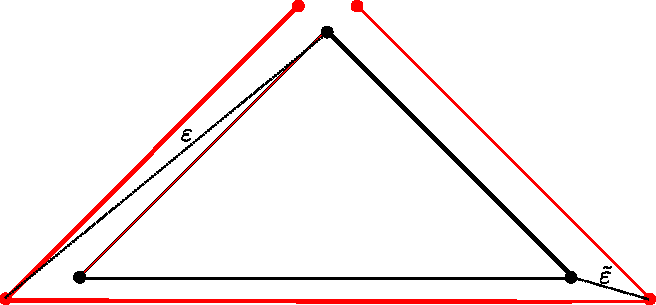
\includegraphics[width=0.8\textwidth]{chapter_2_example_1.pdf}
    \caption{
	    Skizzieren wir zwei Graphen $G_1,G_2$, so zeichnen wir die Knoten und Kanten von $G_1$ stets in schwarz und die Knoten und Kanten von $G_2$ stets in rot.
	    Aufgrund der Konnektivität von $G_1$ induziert die Zuordnung zweier Kanten von $G_1$ auf $G_2$ das Bild der ausbleibenden Zuordnung für die dritte Kante von $G_1$.
	    Die stärker gezeichnete rote Kurve sei hier das Bild einer solchen Graph-Zuordnung von $G_1$ nach $G_2$.
	    Der Flaschenhals-Abstand wird hier durch den (schwachen) Fréchet-Abstand zwischen den stärker gezeichneten Kurven angenommen und ist durch $\varepsilon$ gekennzeichnet.
	    Damit ist $\vec{\delta}_{(w)F}(G_1,G_2) = \varepsilon$.
	    Andersherum tritt ein so großer Flaschenhals-Abstand zum Vergleich nicht auf. Es gilt $\vec{\delta}_{(w)F}(G_2,G_1) = \tilde{\varepsilon}$.
	    \\
	    Im Vergleich zu der \textit{Traversal Distance} von $G_1$ und $G_2$ - einem alternativen Abstandsmaß für eingebetteten Graphen - fällt $\vec{\delta}_{(w)F}(G_1,G_2)$ hier
	    aufgrund der jeweiligen Konnektivität von $G_1$ und $G_2$ deutlich größer aus (siehe dazu Akitaya et. al \cite{Akitaya}, Seite 6).
	    \\
	    \\
	    Quelle: In Anlehnung an Akitaya et. al \cite{Akitaya}, Seite 6, Figure 2 (c).
    }
    \label{chapter_2_example_1}
\end{figure}

Ähnlich wie der (schwache) Fréchet-Abstand beschreibt auch der gerichtete (schwache) Graph-Abstand einen Flaschenhals-Abstand.

\subsection{Lokale Optimierungen}

Generell können für einen konkreten Fall viele Graph-Zuordnungen $s: G_1 \to G_2$ existieren, die den gerichteten (schwachen) Graph-Abstand einhalten.
Im Anwendungsfall kann man sich zum Beispiel mehrere Rekonstruktionen $G_{1,1}, ..., G_{1,n}$ eines Netzwerkes $G_2$ vorstellen.
Anschließend stelle man sich nun die Frage, welche der Rekonstruktionen dem urpsprünglichen Netzwerk $G_2$ am ähnlichsten ist beziehungsweise dieses entsprechend eines konkreten Abstandsmaßes
für Graphen am besten beschreibt.
Der gerichtete (schwache) Graph-Abstand zwischen einem $G_{1i}$ $(i \in \{1,...,n\})$ und $G_2$ beschreibt dabei in gewisser Weise eine obere Schranke für die größte Abweichung zwischen
einer Rekonstruktion $G_{1i}$ und $G_2$.
Unter Umständen haben evlt. sogar alle $G_{1i}$ denselben Flaschenhals-Abstand zu $G_2$, da sie dieselbe entscheidende Abweichung bei der Rekonstruktion von $G_2$ erzeugen.
Insbesondere interessieren wir uns hier nun für die lokale Güte der Rekonstruktion, welche für den gerichteten (schwachen) Graph-Abstand keine Rolle spielt.
\\
\\
Dies motiviert die Einführung eines weiteren Abstandsmaßes auf Graphen, welches auch lokale Optimierungen bei der Zuordnungen der Kanten in Betracht zieht.
\\
\\
Zuvor merken wir an, dass im Allgemeinen eine Graph-Zuordnung $\tilde{s}: G_1 \to G_2$, die jede Kante $e \in E_1$ optimal bezüglich des (schwachen)
Fréchet-Abstands auf $G_2$ abbildet, so dass $\delta_{(w)F}(e, \tilde{s}(e)) \leq \delta_{(w)F}(e, s(e))$, nicht existiert (siehe Abbildung \ref{chapter_2_example_0} für ein Beispiel).

\begin{figure}[H]
    \centering
    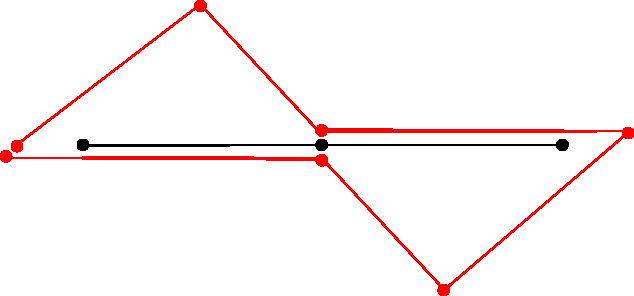
\includegraphics[width=0.8\textwidth]{chapter_2_example_0.pdf}
	\caption{Eine Graph-Zuordnung von $G_1$ nach $G_2$ kann immer nur maximal eine Kante von $G_1$ bezüglich des (schwachen) Fréchet-Abstands optimal zuordnen.
	\\
	\\
	Quelle: In Anlehnung an Figure 2 aus Buchin et. al \cite{Buchin}.
	}
    \label{chapter_2_example_0}
\end{figure}

Alternativ bietet es sich an, die summierten (schwachen) Fréchet-Abstände zwischen den Kanten in $G_1$ und ihren Bildern in $G_2$ unter der Graph-Zuordnung zu optimieren.

\subsection{Optimale Graph-Zuordnungen} \label{Optimale Graphzuordnungen}
Damit widmen wir uns nun dem Abstandsmaß, welches für uns im weiteren Verlauf das Optimalitätskriterum zur Charakterisierung optimaler Zuordnungen auf Graphen beschreibt.

\begin{Def} \label{Definition Min-Sum}
	Min-Sum-Graph-Abstand (engl. min-sum graph distance)

	Wir definieren \textit{Min-Sum}$_{dist}(G_1, G_2)$ als
	$$\min_{s: G_1 \to G_2} \sum_{e \in E_1} dist(e, s(e)),$$
	wobei sich $s$ über alle Graph-Zuordnungen von $G_1$ nach $G_2$ erstreckt und $dist$ ein unspezifisches Abstandsmaß (für den Vergleich von Wegen)
	im euklidischen Raum repräsentiert.
	\\
	\\
	Wählen wir den (schwachen) Fréchet-Abstand als zugrundeliegendes Abstandsmaß, so definieren wir entsprechend
	\textit{Min-Sum}$_{(w)F}(G_1, G_2)$ als $$\min_{s: G_1 \to G_2} \sum_{e \in E_1} \delta_{(w)F}(e, s(e)).$$
	\\
	\\
	Ferner bezeichnen wir mit $Sum_{(w)F}(s) = \sum_{e \in E_1}\delta_{(w)F}(e, s(e))$ die Summe der (schwachen) Fréchet-Abstände zwischen den Kanten
	in $G_1$ und ihren durch $s$ zugeordneten Wegen in $G_2$.
	\\
	Wir nennen $s$ eine Min-Sum$_{(w)F}$ Zuordnung, falls
	\\
	$Sum_{(w)F}(s) = \text{Min-Sum-Graph-Abstand}_{(w)F}(G_1,G_2)$.

\end{Def}

\newpage
\section{Ein polynomieller Algorithmus} \label{Kapitel 3}

In diesem Kapitel werden wir zur Berechnung des Min-Sum$_{(w)F}$ Abstands den Algorithmus aus \cite{Buchin} unter Berücksichtigung einiger relevanter
Begriffe und Ergebnisse aus \cite{Akitaya} herleiten und diesen Algorithmus schließlich anhand eines konkreten Beispiels demonstrieren.
Sei $G_1$ von nun an ein kreisfreier und zusammenhängender Graph, also ein \textit{Baum}.

\subsection{Einschränkungen an die Graph-Zuordnungen} \label{Einschränkungen}
Für die Berechnung von Min-Sum$_{(w)F}(G_1, G_2)$ kommen definitionsgemäß (siehe \ref{Definition Min-Sum}) alle möglichen Graph-Zuordnungen von $G_1$ nach $G_2$ in Betracht.
Im weiteren Verlauf werden wir die Menge der Graph-Zuordnungen jedoch mit zwei Einschränkungen versehen.
Die erste Einschränkung ist dabei optional. Die zweite Einschränkung wird notwendig sein, um die polynomielle Laufzeit des Algorithmus zu gewährleisten.
\\
\\
Bevor wir die Einschränkungen motivieren und beschreiben, wollen wir zunächst weitere Begriffe zur Charakterisierung der Eigenschaften von Graph-Zuordnungen bezüglich
der (schwachen) Fréchet-Abstände zwischen den Kanten von $G_1$ und ihren Bildern in $G_2$ definieren.

\begin{Def}
	$\varepsilon$-Platzierung (engl. $\varepsilon$-Placement)
	Eine \textit{$\varepsilon$-Platzierung eines Knotens $v \in V_1$} ist eine maximal zusammenhängende Komponente von $G_2$ eingeschränkt auf $B_{\varepsilon}(v)$.
	Eine \textit{$\varepsilon$-Platzierung einer Kante $e = \{u,v\} \in E_1$} ist ein Weg $W$ in $G_2$, welcher eine Platzierung $p_u$ von $u$ mit einer Platzierung $p_v$ von $v$
	so verbindet, dass $\delta_F(e, W) \leq \varepsilon$.
	\\
	In diesem Fall nennen wir $p_u$ und $p_v$ \textit{voneinander erreichbar}.
	\\
	Eine \textit{$\varepsilon$-Platzierung von $G_1$} ist eine Graph-Zuordnung $s: G_1 \to G_2$, so dass $s$ jede Kante $e \in G_1$ auf eine $\varepsilon$-Platzierung von $e$ abbildet.
	\\
	Eine schwache $\varepsilon$-Platzierung einer Kante $e = \{u,v\} \in E_1$ ist ein Weg $W$ in $G_2$, welcher eine Platzierung $p_u$ von $u$ mit einer Platzierung $p_v$ von $v$
	so verbindet, dass $\delta_{wF}(e, W) \leq \varepsilon$.
	\\
	In diesem Fall nennen wir $p_u$ und $p_v$ \textit{schwach voneinander erreichbar}.
	\\
	Eine schwache \textit{$\varepsilon$-Platzierung von $G_1$} ist eine Graph-Zuordnung $s: G_1 \to G_2$, so dass $s$ jede Kante $e \in G_1$ auf eine schwache $\varepsilon$-Platzierung von $e$ abbildet.
	Siehe Abbildung \ref{chapter_3_placements_example} für ein Beispiel.
	\\
	\\
	Synonym für $\varepsilon$-Platzierung eines Knotens beziehungsweise einer Kante benutzen wir mitunter auch die Begriffe \textit{Knoten-Platzierung} und \textit{Kanten-Platzierung}.

	\begin{figure}[H]
	    \centering
	    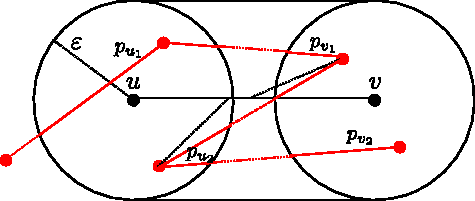
\includegraphics[width=0.8\textwidth]{chapter_3_placements_example.pdf}
		\caption{$B_{\varepsilon}(u)$ enthält zwei $\varepsilon$-Platzierungen von $u$, $p_{u_1}$ und $p_{u_2}$. Analog sind $p_{v_1}$ und $p_{v_2}$
		die $\varepsilon$-Platzierungen von $v$ innerhalb von $B_{\varepsilon}(v)$. Jede Knoten-Platzierung von $G_1$ enthält hier genau einen Knoten von $G_2$.
		Hierbei sind die Paare von Knoten-Platzierungen
		$(p_{u_1},p_{v_1})$, $(p_{u_2},p_{v_1})$ und $(p_{u_2},p_{v_2})$ voneinander erreichbar. Die Bilder möglicher Wege, welche die besagten Paare verbinden, könnten zum Beispiel die
		gezeichneten Kanten in $G_2$ zwischen den (eindeutigen) Knoten innerhalb der entsprechenden Platzierungen sein.
		\\
		\\
		Die schwarz-gepunkteten Geradenstücke haben jeweils Länge $\varepsilon$ und veranschaulichen, dass $p_{u_1}$ und $p_{v_2}$ lediglich schwach voneinander erreichbar sind.
		Sei $W$ ein Weg auf $\{u,v\}$ von $u$ nach $v$ und $X$ ein Weg auf $G_2$ von $p_{u_1}$ nach $p_{v_2}$. Die initiale Orientierung von $W$ und $X$ ist durch jeweils einen Pfeil gekennzeichnet.
		Damit der Abstand zwischen $W$ und $X$ kleiner als $\varepsilon$ ist, sobald $X$ den Knoten $p_{v_1}$ erreicht,
		muss $W$ $\varepsilon$-Ball um $u$ verlassen. Ist $X$ am Knoten bei $p{u_2}$ angekommen ist, muss $W$ zur Einhaltung des $\varepsilon$-Abstands auf $\{u,v\}$ die Orientierung welchseln, da
		der Abstand zwischen dem Knoten bei $p{u_2}$ und einem beliebigen Punkt auf $\{u,v\}$ außerhalb von $B_{\varepsilon}(u)$ größer als $\varepsilon$ ist.
		\\
		\\
		Quelle: Eigene Darstellung.
		}
	    \label{chapter_3_placements_example}
	\end{figure}

\end{Def}

\subsubsection{Erste Einschränkung} \label{Erste Einschränkung}

Wir haben Min-Sum$_{dist}$ allgemein vor dem Hintergrund motiviert, optimale Graph-Zuordnungen auf geometrischen Graphen zu betrachten,
die bereits einen Flaschenhals-Abstand wie den gerichteten (schwachen) Graph-Abstand einhalten.

Um diesen Zusammenhang zu erhalten, werden wir die in Betrachtung zu ziehenden Graph-Zuordnungen zunächst auf die Menge
\begin{center}
	$\{s: G_1 \to G_2 \text{ $|$ } s$ ist eine (schwache) $\varepsilon$-Platzierung von $G_1 \}$
\end{center}
einschränken.
\\
Generell können wir auch $\varepsilon \geq \vec{\delta}_{(w)F}(G_1, G_2)$ fordern, für größere $\varepsilon$ vergrößert sich entsprechend der Freiheitsgrad für die
in Betrachtung zu ziehenden Graph-Zuordnungen, womit sich potentiell Min-Sum$_{(w)F}(G_1, G_2)$ verringert.
\\
Wir merken an dieser Stelle an, dass eine $\varepsilon$-Platzierung von $G_1$ nach $G_2$ für $\varepsilon < \vec{\delta}_{(w)F}(G_1,G_2)$
nicht existieren kann. Dies folgt direkt aus den Definitionen \ref{Definition Graph-Abstand} und \ref{Definition Min-Sum}.

\subsubsection{Zweite Einschränkung} \label {Zweite Einschränkung}
Da wir hier zur Berechnung der Abstände zwischen einer Kante $\{u,v\} \in E_1$ und ihrem Bild $s(\{u,v\})$ unter einer Graph-Zuordnung $s$ den (schwachen) Fréchet-Abstand verwenden,
hat die Wahl der Bilder $s(u)$ und $s(v)$, innerhalb der entsprechenden $\varepsilon$-Platzierungen von $u$ und $v$, eine direkte Auswirkung auf die summierten Abstände.
Anders ausgedrückt: Im Gegensatz zu $\vec{\delta}_{(w)F}(G_1,G_2)$ ist Min-Sum${(w)F}(G_1,G_2)$ nicht invariant unter dem Freiheitsgrad, den $s$
bei der Wahl der Bildpunkte $s(u)$ und $s(v)$ unter Einhaltung des (schwachen) Fréchet-Abstands hat. Siehe \ref{chapter_3_example_0} für ein konkretes Beispiel.

\begin{figure}[H]
    \centering
    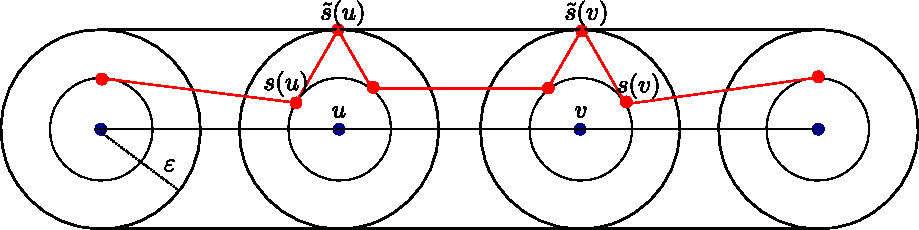
\includegraphics[width=\textwidth]{chapter_3_example_0.pdf}
	\caption{Die Wahl der Randpunkte $\tilde{s}(u), \tilde{s}(v)$ für das Bild der mittleren Kante $\{u,v\}$ ermöglicht zwar eine $\varepsilon$-Platzierung
	für den skizzierten Graphen, allerdings ist diese nicht optimal bezüglich des Min-Sum$_{(w)F}$ Abstands .
	Die (schwachen) Fréchet-Abstände zwischen einer Kante und ihrem Bild betragen unter $\tilde{s}$ jeweils $\varepsilon$.
	Unter $s$ hingegen wird der Flaschenhals-Abstand von $\varepsilon$ nur durch die Platzierung der mittleren Kante angenommen.
	Die äußeren Kanten lassen sich so platzieren, dass der (schwache) Fréchet-Abstand nur $\frac{\varepsilon}{2}$ beträgt.
	\\
	\\
	Quelle: In Anlehnung an eine unveröffentlichte Bemerkung und Skizze der Autoren von \cite{Buchin}.
	}
    \label{chapter_3_example_0}
\end{figure}

Um diesen Freiheitsgrad und die dadurch implizierte Komplexität bezüglich der Berechnung von Min-Sum$_{(w)F}(G_1,G_2)$ auszuschließen,
werden wir für einen Knoten $u \in V_1$ sein Bild unter einer Graph-Zuordnung für jede seiner $\varepsilon$-Platzierung fixieren.
Als Fixpunkt wählen wir dafür einen Punkt innherhalb der $\varepsilon$-Platzierung mit minimalem Abstand zu $u$.
Wir behaupten (ohne Beweis), dass die Berechnung von Min-Sum$_{(w)F}(G_1,G_2)$ ohne eine solche Einschränkung im Allgmeinen NP-schwer ist.

\subsection{Ansätze und Beschreibung eines polynomiellen Algorithmus} \label{Grundidee des Algorithmus}
Um unter den Einschränkungen \ref{Erste Einschränkung} und \ref{Zweite Einschränkung} an die zu betrachtenden Graph-Zuordnungen von $G_1$ nach $G_2$
Min-Sum$_{(w)F}(G_1,G_2)$ zu berechnen, wollen wir eine
eine $\varepsilon$-Platzierung $s: G_1 \to G_2$ konstruieren, die das Optimalitätskriterium (siehe \ref{Optimale Graphzuordnungen}) erfüllt.
Für eine solche Abbildung $s$ gilt dann entsprechend $\sum_{e \in E_1}\delta_{(w)F}(e, s(e)) = \text{Min-Sum}_{(w)F}(G_1,G_2)$.
\\
\\
Der algorithmische Ansatz zur Lösung des Entscheidungsproblems, ob eine $\varepsilon$-Platzierung von $G_1$ existiert (siehe [2] Seiten 9-11), liefert das
Grundgerüst für die Konstruktion von $s$. Wir wollen diesen algorithmischen Ansatz motivieren und die Berechnungsschritte im Detail beschreiben.
Der Algorithmus gliedert sich in insgesamt 4 Einzelschritte, die wir im Verlauf des Kapitels entsprechend kennzeichnen werden.

\subsubsection{$\varepsilon$-Platzierungen der Knoten} \label{Platzierungen der Knoten}
Die Zuordnung der Knoten $u,v \in V_1$ auf einen Punkt jeweils innerhalb ihrer $\varepsilon$-Platzierungen bedingt die Randpunkte $W(0)$, $W(1)$
für einen einfachen Weg $W: [0,1] \to G_2$, auf den die Kante $\{u,v\} \in E_1$ durch eine Graph-Zuordndung $s$ abgebildet werden kann.
Dass diese Randpunkte innerhalb der $\varepsilon$-Platzierung ihrer jeweiligen Knoten liegen, ist ein notwendiges Kriterium dafür, dass der (schwache) Fréchet-Abstand
zwischen der Kante und ihrem Bild unter $s$ nicht größer als $\varepsilon$ ist.

Aus der Definition des (schwachen) Fréchet-Abstands (siehe \ref{Definition Fréchet-Abstand}) folgt direkt, dass
$\delta_{(w)F}(e, W) \geq max{\{\|u-W(0)\|, \|v-W(1)\|\}}$.
\\
\\
Anfangs berechnen wir zunächst alle $\varepsilon$-Platzierungen der Knoten in $G_1$ und bezeichnen für einen Knoten $v \in V_1$ mit $P(v)$ die Menge
aller $\varepsilon$-Platzierungen von $v$.

\subsubsection{Schritt 1} \label{Schritt 1}
TODO: Laufzeiten
\\
\\
Wir initialisieren $\varepsilon$ mit $\varepsilon \geq \vec{\delta}_{(w)F}(G_1, G_2)$.
Da $G_1$ ein Baum ist, können wir
$\vec{\delta}_{wF}(G_1, G_2)$ in $O(...)$ und $\vec{\delta}_F(G_1, G_2)$ in $O(...)$ berechnen. Siehe dazu (...)
Anschließend berechnen wir die $\varepsilon$-Platzierungen aller Knoten von $G_1$. Jeder Knoten in $G_1$ hat $O(m_2)$
$\varepsilon$-Platzierungen, womit insgesamt $(n_1*m_2)$ $\varepsilon$-Platzierung zu berechnen sind.
Für jeden Knoten lassen sich seine $\varepsilon$-Platzierungen über einen Standard-Algorithmus zur Berechnung von
zusammenhängenden Komponenten in Graphen ermitteln, dessen Laufzeit linear in der Größe von $G_2$ ist.
Die Laufzeit - und Speicherkomplexität beträgt somit $O(n_1*m_2)$.

\subsubsection{Schritt 2} \label{Schritt 2}
Für jede Kante $\{u, v\} \in E_1$ berechnen wir nun die (schwachen) Erreichbarkeiten zwischen den $\varepsilon$-Platzierungen der Knoten von $u,v$.
Dabei ist für jede Kombination $p_u, p_v$ von $\varepsilon$-Platzierungen von $u$ und $v$ zu jeweils zu entscheiden, ob sie (schwach) voneinander erreichbar sind.

Um nur die schwache Erreichbarkeit zu entscheiden, ist die Existenz eines einfachen Weges zwischen zwei Knoten-Platzierungen
$p_u,p_v$, welcher vollständig innerhalb von $T_{\varepsilon}(\{u,v\})$ liegt, bereits ein hinreichendes Kriterium (siehe [3], Seite 83).
z
Schränken wir $G_2$ auf $T_{\varepsilon}(\{u,v\})$ ein, so sind alle Knoten-Platzierungen innerhalb derselben zusammenhängenden Komponente von $G_2$
schwach voneinander erreichbar. Entsprechend speichern wir für eine zusammenhängende Komponente von $G_2$ innerhalb $T_{\varepsilon}(e)$ jeweils zwei Listen mit den
zusammenhängenden Knoten-Platzierungen von $u$ und $v$.

Die schwachen Erreichbarkeiten zwischen allen Knoten-Platzierungen entlang einer Kante in $G_1$ lassen sich somit mit einer Laufzeit von $O(m_2)$ berechnen.
Insgesamt beträgt die Zeit - und Speicherkomplexität zur Berechnung der Erreichbarkeiten aller Kanten in $G_1$ $O(m_1*m_2)$.
\\
\\
Für den Fréchet-Abstand ist die Existenz eines einfachen Weges $W$ innerhalb von $T_{\varepsilon}(\{u,v\})$, welcher $p_u$ und $p_v$ miteinander verbindet,
zwar ein notwendiges aber kein hinreichendes Kriterium dafür, dass $p_u$ und $p_v$ voneinander erreichbar sind. Wir müssen für $W$ explizit entscheiden,
ob $\delta_F(\{u,v\}, W) \leq \varepsilon$.
\\
\\
Dabei können wir für zwei Wege $Y$ und $Z$ das Entscheidungsproblem $\delta_F(Y,Z) \leq \varepsilon$ in $O(|Y|*|Z|)$ lösen (siehe dazu \cite{Alt}, Seite 77).
Da $\{u,v\}$ ein Geradenstück ist, hat $\{u,v\}$ die Länge $1$. Damit können wir die Erreichbarkeit zwischen $\{u,v\}$ und $W$ in $O(|W|)$ entscheiden.
Da $W$ per Bedingung ein einfacher Weg ist, besteht $W$ aus maximal $m_2$ Kanten (beziehungsweise Teilkanten) von $G_2$.
Zur Speicherung der Erreichbarkeiten speichern wir für jede $\varepsilon$-Platztierung von $u$ eine Liste mit $\varepsilon$-Platzierungen von $v$, die
über einen Weg voneinander erreichbar sind. Um die Liste für ein $p_u \in P(u)$ zu berechnen, starten wir eine Graph-Suche zur Ermittlung eines
Weges in $G_2$ beginnend bei $p_u$. Verlassen wir während der Suche entweder $T_{\varepsilon}(\{u,v\})$ beziehungsweise überschreitet der Fréchet-Abstand $\varepsilon$,
so entfernen wir den Suchzweig aus der Liste der möglichen Abeziehungsweiseigungen in $G_2$.
Für eine Kante in $G_1$ beträgt die Laufzeit der Suche somit $O(m_2^2)$ und pro Kante zählen wir bis zu $m_2^2$ Paare von potentiell voneinander erreichbarer Knoten-Platzierungen.
Für alle Kanten in $G_1$ liegt die Speicher - und Laufzeitkomplexität damit bei $O(m_1*m_2^2)$.

\subsubsection{Existenz einer $\varepsilon$-Platzierung von $G_1$}
Bis zu diesem Schritt haben wir die (schwachen) Erreichbarkeiten zwischen Knoten-Platzierungen paarweise ermittelt.
Nun wollen wir unseren Wortschatz um den Begriff der Knoten-Platzierungen um eine Eigenschaft erweitern, um anschließend eine Aussage über die Existenz
einer $\varepsilon$-Platzierung von $G_1$ treffen zu können.
\\
Hat ein Knoten $u \in V_1$ neben $\{u,v\} \in E_1$ noch eine weitere inzidente Kante $\{u,w\}$, so muss neben einem $p_v \in P(v)$ insbesondere auch
ein $p_w \in P(w)$ existieren, so dass die Paare $(p_u,p_v)$ und $(p_v,p_u)$ jeweils (schwach) voneinander erreichbar sind. Die (schwache) Erreichbarkeit
zwischen einer Knoten-Platzierungen mit mindestens einer Knoten-Platzeriung benachbarter knoten stellt somit ein notwendiges Kriterium für die Existenz
einer $\varepsilon$-Platzierung von $G_1$ dar und motiviert damit die folgende Definition.

\begin{Def}
	Gültige $\varepsilon$-Platzierung (engl. valid placement)
	Eine $\varepsilon$-Platzierung $p_v$ eines Knotens $v$ nennen wir (schwach) \textit{gültig}, falls für jeden Nachbarn $u$ von $v$
	eine $\varepsilon$-Platzierung $p_u$ existiert, so dass $p_v$ und $p_u$ (schwach) voneinander erreichbar sind.
	Ansonsten nennen wir $p_v$ (schwach) ungültig.
\end{Def}

Für die Konstruktion von $s$ dürfen wir nur (schwach) gültige $\varepsilon$-Platzierungen der Knoten von $G_1$ betrachten, denn die
Wahl einer ungültigen Knoten-Platzierung schließt definitionsgemäß direkt aus, dass $s$ eine $\varepsilon$-Platzierung von $G_1$ sein kann.
Entsprechend löschen wir unter den in Schritt 1 ermittelten Knoten-Platzierungen alle diejenigen, die (schwach) ungültig sind.
\\
\\
Dabei ist zu beachten, dass nach dem Löschen einer (schwach) ungültigen $\varepsilon$-Platzierung von $v \in P(v)$
jede vor der Löschung noch (schwach) gültige $\varepsilon$-Platzierung eines Nachbarn von $v$ nun (schwach) ungültig geworden sein kann.
Unter Umständen war zum Beispiel die Gültigkeit der Knoten-Platzierung eines Nachbarn von $v$ gerade durch die Erreichbarkeit zu der zuvor gelöschten
$\varepsilon$-Platzierung von $v$ bedingt.
In dem Sinne löschen wir rekursiv solange (schwach) ungültige $\varepsilon$-Platzierungen der Knoten in $G_1$, bis
keine (schwach) ungültigen Knoten-Platzierungen mehr existieren. Als Abbruchbedingung der Rekursion gilt daher, dass die Löschung der letzten bekannten
ungültigen Knoten-Platzierung keine weitere Löschung mehr impliziert.

\subsubsection{Schritt 3} \label{Schritt 3}
In diesem Schritt werden wie oben beschrieben alle Knoten-Platzierungen (rekursiv) bereinigt.
Um für eine Kante $\{u,v\} \in E_1$ zu entscheiden, welche Platzierungen der Knoten $u$ und $v$ voneinander (schwach) erreichbar sind, bedienen wir uns dafür der in
Schritt 2 berechneten Erreichbarkeiten. In Schritt 1 haben wir $O(n_1*m_2)$ Knoten Platzierungen ermittelt.

Für die schwache Erreichbarkeit haben wir in Schritt 2 für eine Kante $\{u,v\} \in E_1$ die zusammenhängende Komponente innerhalb von $T_{\varepsilon}(\{u,v\})$
und ihre enthaltenen Knoten-Platzierungen von $u$ und $v$ gespeichert.
\\
Ist nun eine Knoten-Platzierung $p_v \in P(v)$ ungültig, so muss $p_v$ aus allen entsprechenden Listen von Knoten-Platzierungen gelöscht werden, in
denen $p_v$ enthalten ist. Dies betrifft potentiell alle zu $v$ adjazenten Knoten, daher beträgt die Laufzeit zum Bereinigen von $p_v$ $O(deg(v))$.
Mit der Identität $\sum_{v \in V_1}(deg(v)) = 2m_1$ beträgt die Laufzeit zum Bereinigen aller ungültigen Knoten-Platzierungen $O(m_1*m_2)$.
\\
Für die nicht-schwache Erreichbarkeit haben wir für jede Knoten-Platzierung $p_v$ eine Liste mit erreichbaren Knoten-Platzierungen gespeichert.
Sollte $p_v$ ungültig sein, so müssen wir $p_v$ für jeden zu $v$ adjazenten Knoten aus den Listen der Knoten-Platzierungen entfernen, in denen $p_v$ enthalten ist.
Für jeden ajdazenten Knoten sind dies $O(m_2)$ Listen, daher beträgt die Laufzeit für die Löschung von $p_v$ insgesamt $O(deg(v)*m_2)$.
Das Bereinigen aller Knoten-Platzierungen beträgt entsprechend $O(m_1*m_2^2)$.
\\
\\
Nachdem Schritte 1-3 durchgeführt wurden, liefert uns ein Hilfssatz aus Akitaya et al. (siehe dazu Seite 13. Lemma 6) eine verbindliche Aussage über die Existenz
einer (schwachen) $\varepsilon$-Platzierung von $G_1$:

\begin{Lem} \label {Lemma 1}
	Sei $G_1$ ein Baum und für $v \in V_1$ sei $\tilde{P}(v)$ die Menge der (schwach) gültigen $\varepsilon$-Platzierungen von $v$, nachdem
	alle (schwach) ungültigen $\varepsilon$-Platzierungen der Knoten in $G_1$ rekursiv gelöscht wurden (analog wie in \ref{Schritt 3}).
	Enthält $\tilde{P}(v)$ für jedes $v \in V_1$ mindestens eine (schwach) gültige $\varepsilon$-Platzierung, so existiert
	eine (schwache) $\varepsilon$-Platzierung von $G_1$.
\end{Lem}

\begin{proof}
Für den Beweis konstruieren wir eine $\varepsilon$-Platzierung von $G_1$.
Wir ernennen einen beliebigen Knoten $v_r \in V_1$ zur Wurzel und betrachten $G_1$ als gerichteten Baum (Out-Tree) ausgehend von $v_r$ .
Wir ordnen $v_r$ einen beliebigen Punkt innerhalb einer seiner (schwachen) $\varepsilon$-Platzierung zu und bearbeiten anschließend iterativ alle
Knoten in $G_1$ ausgehend von der Wurzel $v_r$.

Dabei wählen wir stets für einen Knoten $v \in V_1$, dessen Vorgänger bereits zugewiesen wurde,
die $\varepsilon$-Platzierung $p_v \in P(v)$ von $v$ so, dass $p_v$
und die bereits ausgewählte (beziehungsweise zugeordnete) $\varepsilon$-Platzierung $p_a$ des Vorgängers von $v$ voneinander (schwach) erreichbar sind.
Für die Kante zwischen $v$ und seinem Vorgänger können wir nun eine passende Kanten-Platzierungen wählen.
\\
Nach Vorraussetzung ist $p_a$ (schwach) gültig und somit muss ein $p_v$ mit der geforderten Erreichbarkeit zu $p_a$ existieren.
Per Definition der (schwachen) Erreichbarkeit gilt, dass mindestens ein einfacher Weg in $G_2$ existiert, welcher $p_v$ und $p_a$ verbindet
und dessen (schwacher) Fréchet-Abstand mit der Kante zwischen $v$ und seinem Vorgänger nicht größer als $\varepsilon$ ist.
Einen solchen Weg wählen wir nun als $\varepsilon$-Platzierung für die Kante zwischen $v$ und seinem Vorgänger.
\\
Da wir $G_1$ als gerichteten Baum betrachten, sind nach endlich vielen Schritten ausgehend von der Wurzel ausgehend alle Knoten in $G_1$
entsprechend zugewiesen und ihre $\varepsilon$-Platzierungen
wurden mit den $\varepsilon$-Platzierungen ihrer Vorfahren durch einen einfachen Weg in $G_2$ verbunden.
Da $G_1$ als Baum insbesondere kreisfrei ist, konnte so jede Kante explizit in $G_1$ einer $\varepsilon$-Platzierung zugeordnet werden.
Die durch die Auswahl dieser $\varepsilon$-Platzierungen implizierte Graph-Zuordnung ist damit insgesamt eine $\varepsilon$-Platzierung von $G_1$.
\end{proof}

Über die Konstruktion aus dem Beweis von Lemma \ref{Lemma 1} erhalten wir einen ersten Ansatz zur Konstruktion einer $\varepsilon$-Platzierung gemäß der Einschränkungen und
des Optimalitätskriteriums.

\subsubsection{Optimale Kanten-Platzierungen}
Im Beweis von $\ref{Lemma 1}$ konnten wir zur Konstruktion einer $\varepsilon$-Platzierung von $G_1$ stets eine beliebige $\varepsilon$-Platzierung einer Kante wählen.
\\
\\
Diesen Ansatz werden wir erweitern, indem wir statt einer beliebigen jeweils nur eine lokal optimale $\varepsilon$-Platzierung einer Kante für die Graph-Zuordnung in Betracht ziehen.
Dabei minimiert eine lokal optimale Kanten-Platzierung $p_{\{u,v\}}$ den (schwachen) Fréchet-Abstand zu der Kante $\{u,v\}$.
Für ein paar Knoten-Platzierungen $p_u, p_v$ sei $$\Delta(p_u,p_v) = \min_{p_{{\{u,v}\}}} \delta_{(w)F}(\{u,v\},p_{\{u,v\}}),$$ wobei sich $p_{{\{u,v}\}}$ über alle
$\varepsilon$-Platzierungen von $\{u,v\}$ erstreckt. Die unter \ref{Zweite Einschränkung} geforderten Fixpunkte werden dafür vor der Berechnung von $\Delta$ gesetzt.

Wir erweitern Schritt 2 des Algorithmus um die Berechnung optimaler Kanten-Platzierungen und speichern für jede Kante $e=\{u,v\} \in G_1$ eine Liste $L_e$
mit Einträgen $(p_v, p_u, \Delta(p_v,p_v))$ für alle $p_v \in P(v)$, $p_u \in P(u)$ die (schwach) voneinander erreichbar sind.
\\
\\
Sofern $L_e$ für alle Knoten in $G_1$ berechnet ist und alle ungültigen Knoten-Platzierungen nach Ausführung von Schritt 3 (\ref{Schritt 3}) bereinigt sind,
reduziert sich die Konstruktion einer optimalen $\varepsilon$-Platzierung auf eine optimale Gesamt-Auswahl der jeweiligen Paare von Knoten-Platzierungen für jedes Paar adjazenter Knoten in $G_1$.
So eine Konstruktion ließe sich analog wie im Beweis zu Lemma $\ref{Lemma 1}$ realisieren und eine so ermittelte Graph-Zuordnung ist insbesondere auch eine $\varepsilon$-Platzierung von $G_1$.
Letztlich stellt dann die Frage, unter welcher der möglichen Auswahlen von Knoten-Platzierungen bei der Konstruktion von $s$ die Summe der Gewichte der durch $s$ implizierten Kanten-Platzierungen
minimiert und damit das Optimalitätskriterium erfüllt wird.

\subsubsection{Konstruktion einer optimalen $\varepsilon$-Platzierung von $G_1$}
Ein naiver Ansatz zur Berechnung von Min-Sum$_{(w)F}(G_1,G_2)$ wäre nun, alle möglichen Kombinationen der $\varepsilon$-Platzierungen der Knoten von $G_1$ über zum Beispiel einen Backtracking-Algorithmus auszuschöpfen.
Dabei würden wir - beginnend bei dem ausgewiesenen Wurzelknoten $v_r$ - die Knoten und Kanten von $G_1$ wie in der Konstruktion der Graph-Zuordnung (siehe $\ref{Lemma 1}$) zuordnen.
An jedem Knoten, wo es für die Auswahl einer Knoten-Platzierung mehr als eine Möglichkeit gibt, hätte der Backtracking-Algorithmus eine Abeziehungsweiseigung pro möglicher Auswahl.
Sobald wir erstmalig $G_1$ vollständig zugeordnet haben, speichern wir die Zuordnung $s$ sowie ihr Gewicht $Sum_{(w)F}(s)$, welches sich als Summe der
paarweise gewählten Knoten-Platzierungen und ihren $\Delta$-Gewichten ergibt.
Für einen bereits zugeordneten Teilgraphen könnten wir sein Gewicht unter den bereits zugeordneten Kanten mitführen und backtracken, sobald dieses das bis zu diesem Iterationsschritt
minimalste Gewicht einer vollständigen Zuordnung von $G_1$ überschreitet. Nachdem der Algorithmus terminiert, hätten wir so Min-Sum$_{(w)F}(G_1,G_2)$ berechnet.
\\
\\
Allerdings ist trotz der Einschränkungen an die zu betrachteten Graph-Zuordnungen der Möglichkeitenraum im Allgemeinen zu groß
für einen solchen (brute-force) Ansatz.
Jeder Knoten in $G_1$ hat potentiell bis zu $m_2$ $\varepsilon$-Platzierungen und für
zwei benachbarte Knoten in $G_1$ gibt somit bis zu $m_2^2$ Möglichkeiten, die Knoten-Platzierungen zu kombinieren.
Insgesamt wächst die Anzahl der potentiellen Kombinationsmöglichkeiten exponentiell mit der Anzahl der Kanten beziehungsweise der Anzahl der Knoten(**) von $G_1$.
(**) Da $G_1$ ein Baum ist, gilt $m_1 = n_1-1$.
\\
\\
Im letzten Schritt des Algorithmus konstruieren wir eine geeignete Suchstruktur für die Zuweisung und Gewichtung von Knoten-Platzierungen.
Dabei werden wir die Knoten-Platzierungen \textit{greedy} berechnen und auswählen.
Anschließend werden wir eine $\varepsilon$-Platzierung $s$ konstruieren, die ebenfalls eine Min-Sum$_{(w)F}$ Zuordnung ist, also das Optimalitätskriterium erfüllt.
\\
\\
\subsubsection{Schritt 4}
Wir interpretieren $G_1$ nach wie vor (analog wie im Beweis zu Lemma \ref{Lemma 1}) als gerichteten Wurzelbaum  mit beliebiger Wurzel $v_r$ und
konstruieren einen abstrakten Graphen $H = (V_H, E_H)$ als Suchstruktur für die Berechnung.
Jede (gültige) $\varepsilon$-Platzierung $p_v$ eines Knotens $v \in V_1$ wird durch einen entsprechenden Knoten $i_{p_v} \in V_H$ repräsentiert.
Für zwei Knoten-Platzierungen $p_v \in P(v)$ und $p_u \in P(u)$ gilt $(i_{p_u},i_{p_v}) \in E_H$ genau dann, wenn

\begin{enumerate}
	\item[(i)] $G_1$ die (gerichtete) Kante $(v,u)$ enthält und
	\item[(ii)] $p_v$ und $p_u$ (schwach) voneinander erreichbar sind.
\end{enumerate}

Insgesamt ist $H$ somit ein gerichteter, azyklischer Graph. Die Gerichtetheit folgt dabei direkt aus der Konstruktion der Kanten in $H$ und
ein Kreis in $H$ würde direkt der Vorraussetzung widersprechen, dass $G$ ein (gerichteter) Baum ist.
Da jeder Knoten in $G_1$ bis zu $m_2$ Knoten-Platzierungen hat, gilt $|V_H| \in O(n_1*m_2)$ und $|E_H| \in O(n_1*m_2^2)$.
\\
Wir induzieren durch $w_H: E_H \to \mathbb{R}$ mit $w_H(i_{p_v},i_{p_u}) = \Delta(p_v,p_v)$ eine Gewichtung der Kanten von $H$ und
initialisieren $w(p_v) = 0$ für alle Knoten-Platzierungen.
Wir werden nun die Knoten-Platzierungen iterativ und greedy einander zuweisen und so eine optimale $\varepsilon$-Platzierung von $G_1$ berechnen.
Im Gegensatz zu der Konstruktion von Lemma \ref{Lemma 1} berechnen wir $s$ und die Gewichte der Knoten-Platzierungen \textit{bottom-up}.
Für einen Knoten $v \in V_1$, dessen Nachfahren ausschließlich Blätter in $G_1$ sind, setzen wir

\begin{equation}
	w(p_v) = \sum_{\text{$u:$ $u$ ist Nachfahre von $v$}} \min_{p_u \in P(u)} w(p_u) + w_H(p_v,p_u) \label{optimal placements}
\end{equation}

Dabei speichern wir die Zuordnung $s$ welche $w(p_v)$ realisiert für alle $p_v \in P(v)$ und löschen alle Nachfahren von $v$ aus $G_1$,
nachdem alle Knoten-Platzierungen von $v$ bearbeitet wurden.
Diese Bearbeitung eines Knotens in $G_1$ bezeichnen wir als einen Iterationsschritt \label{Iterationsschritt}

\begin{Lem} \label{Lemma 2}
	Schritt 4 berechnet in $O(n_1)$ Iterationsschritten (siehe \ref{Iterationsschritt}) $\text{Min-Sum}_{(w)F}(G_1,G_2)$ und
	eine optimale $\varepsilon$-Platzierung von $G_1$.
\end{Lem}

\begin{proof}
Wir beweisen die Aussage über die Invariante, dass nach jedem Iterationsschritt der Teilgraph (eingeschränkt auf
den zuletzt bearbeiteten Knoten) optimal zugeordnet ist.

Vor dem ersten Iterationsschritt ist das Gewicht aller Knoten-Platzierungen $0$.
Wir bezeichnen den aktualisierten Graphen $G_1$ nach dem $i$-ten Iterationsschritt mit $G_1^i$.
Für einen beliebigen Knoten $v \in V_1$, dessen Nachfahren Blätter in $G_1^0$ sind, wird das Gewicht aller Knoten-Platzierungen nun durch die Berechnung von Gleichung (\ref{optimal placements})
für alle Nachfahren von $v$ minimiert. Insbesondere entspricht $w(v)$ gerade der Summe aller gewichteten Kanten-Platzierungen. Betrachten wir nun $s$ als die Abbildung, die $\min{w(p_v)}: p_v \in P(v)$ realisiert,
so ist $s$ offensichtlich eine Graph-Zuordnung, die Min-Sum$_{(w)F}(G_v, G_2)$ auf dem Teilgraphen $G_v$ - mit $v$ als Wurzel - einhält.
\\
Seien nun alle Teilgraphen in $G_1^i$ für ein beliebiges $i>1$ an allen bereits bearbeiteten Knoten optimal zugeordnet und sei $u \in V_1$ ein Knoten, dessen
Nachfahren Blätter in $G_1^i$ sind. Die Graph-Zuordnung, die $\min{w(p_u)}: p_u \in P(u)$ realsiert, wählt unter Umständen nach der Berechnung von \ref{optimal placements}
für einen Nachfahren $\tilde{u}$ von $u$ eine andere Knoten-Platzierung als $\min{w(p_{\tilde{u}}}): p_{\tilde{u}} \in P(\tilde{u})$. Nach Vorraussetzung sind jedoch
wiederum alle (potentiellen) Nachfahren von $\tilde{u}$ für jede Knoten-Platzierung von $\tilde{u}$ optimal zugeordnet. Insgesamt ist damit die Graph-Zuordnung, die $\min{w(p_u)}: p_u \in P(u)$ realisiert,
optimal in dem geforderten Sinne.
\\
\\
Da zu Beginn von Schritt 4 weniger als $n_1$ Knoten mindestens einen Nachfahren haben und pro Iteration genau ein Knoten bearbeitet wird,
ended Schritt 4 nach $O(n_1)$ Iterationsschritten mit der Berechnung der Wurzel $v_r$ und es gilt nach obiger Argumentation:
\begin{equation}
	\min_{p_{v_r} \in P(v_r)}{w(p_{v_r})} = \text{Min-Sum}_{(w)F}(G_1,G_2) \label {last one}
\end{equation}
Die Gleichung (\ref{last one}) realisierende Graph-Zuordnung ist (nach \ref{Lemma 1}) eine $\varepsilon$-Platzierung von $G_1$.
\\
\end{proof}

Insgesamt setzt sich der Algorithmus also aus den folgenden Einzelschritten zusammen:
\begin{enumerate}
	\item[1)] Schritt 1: Berechnung der $\varepsilon$-Platzierungen der Knoten von $G_1$
	\item[2)] Schritt 2: Berechnung der (schwachen) Erreichbarkeiten und optimaler Kanten-Platzierungen
	\item[3)] Schritt 3: Löschung aller ungültigen $\varepsilon$-Platzierungen der Knoten von $G_1$
	\item[4)] Schritt 4: Konstruktion der Suchstruktur $H$ und iterative Berechnung von Min-Sum$_{(w)F}(G_1, G_2)$ und einer optimalen $\varepsilon$-Platzierung von $G_1$.
\end{enumerate}

\begin{Satz}
	Sei $G_1$ ein Baum und sei $\varepsilon \geq \vec{\delta}_{(w)F}(G_1,G_2)$.
	So lässt sich unter Einhaltung der Einschränkung \ref{Zweite Einschränkung} eine $\varepsilon$-Platzierung $s$ von $G_1$
	mit einer polynomiellen Laufzeitkomplexität von $O(n_1*m_2^3) + T_{(w)F}(g_1, g_2)$ und einer polynomiellen Speicherkomplexität von $O(n_1*m_2^2) + S_{(w)F}(g_1, g_2)$ berechnen, so dass für jede
	andere $\varepsilon$-Platzierung $\tilde{s}$ von $G_1$ gilt:
	$$\sum_{e \in E_1}\delta_{(w)F}(e, s(e)) \leq \sum_{e \in E_1}\delta_{(w)F}(e, \tilde{s}(e)).$$
	Dabei beschreibt $T_{(w)F}(g_1, g_2)$ die Laufzeitkomplexität und $S_{(w)F}(g_1, g_2)$ die Speicherkomplexität zur Berechnung der minimalen (schwachen) Fréchet-Abstände, in Abhängigkeit
	der durch $g_1$ und $g_2$ symbolisierten Komplexitäten von $G_1$ und $G_2$.
\end{Satz}

\begin{proof}
Die Korrektheit des Algorithmus folgt direkt mit Lemma \ref{Lemma 2}.
Zur Berechnung des minimalen (schwachen) Fréchet-Abstands existieren in der Literatur diverse Algorithmen mit unterschiedlichen polynomiellen Laufzeit - und Speicherkomplexitäten.
Diese wollen wir hier lediglich referenzieren. Entscheidend für uns ist, das entsprechend Laufzeit - und Speicherkomplexiäten zum Berechnen des Problems tatsächlich polynomiell sind.
Für den Fréchet-Abstand verweisen wir hierfür konkret auf Alt et. al \cite{Alt2} (Seite 272). Weitere polynomielle Ansätze finden sich zusätzlich in \cite{Ref1} und \cite{Ref2}.
\\
Ansonsten wird die sonstige Speicherkomplexit der Schritte 1-4 durch die Speicherung von $H$ und die sonstige Laufzeitkomplexität der Schritte 1-4 durch die Berechnung von
Gleichung (\ref{last one}) dominiert.
\\
$H$ speichert alle Paare (schwach) voneinander erreichbarer Knoten-Platzierungen sowie die minimalen (schwachen) Fréchet-Abstände zwischen einem sie verbindenden Weg
und der assoziierten Kante in $G_1$. Für zwei (schwach) voneinander erreichbare Knoten-Platzierungen enthält $H$ eine Kante. Für jeden Knoten in $G_1$ gibt es $O(m_2^2)$ solcher Paare
und insgesamt liegt die Speicherkomplexität von $H$ für alle Knoten in $G_1$ damit bei $O(n_1*m_2^2)$.
\\
Zur Berechnung von Gleichung (\ref{last one}) betrachten wir für eine feste Knoten-Platzierung $p_v \in P(v)$ den zur Lösung der Gleichung relevanten Teilgraphen von $H$,
bestehend aus allen Knoten-Platzierungen von $v$ sowie deren (schwach) erreichbaren Nachfahren. Dieser Teilgraph weist somit für eine fixierte Knoten-Platzierung eine Komplexität von $O(m_2^2)$ auf.
Sofern $v$ nicht die Wurzel ist, gibt es $deg(v)-1$ Nachfahren von $v$. Ferner gilt $|P(v)| \in O(m_2)$. Damit beträgt die Zeitkomplexität zur Berechnung von Gleichung (\ref{last one}) für alle
Knoten-Platzierungen von $v$ insgesamt

\begin{equation}
	O(deg(v)*m_2^3).
\end{equation}
Mit (2) und der Identität
\begin{equation}
	\sum_{v \in V_1} deg(v) = 2*m_1 = 2(n-1)
\end{equation}
ergibt sich schließlich die Laufzeitkomplexität von $O(n_1*m_2^3).$
\end{proof}
\newpage

\subsection{Ein Beispiel}
Anhand eines kleinen Beispiels (siehe Abbildung \ref{min_sum_tree_0}) wollen wir den oben beschriebenen Algorithmus nun demonstrieren.

\begin{figure}[H]
    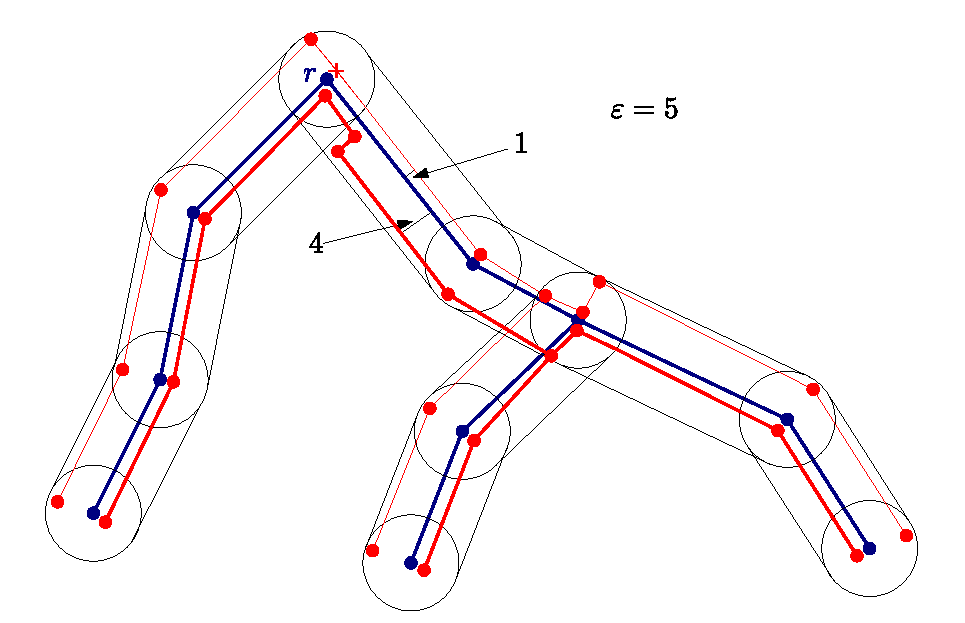
\includegraphics[width=\textwidth]{min_sum_tree_0.pdf}
	\caption{
	$G_1$ ist in schwarz und $G_2$ in rot gezeichnet. Der Wurzelknoten für $G_1$, welcher die Bearbeitungsreihenfolge der Knoten für den Algorithmus sowie die Struktur
	des Suchgraphen $H$ bestimmt, ist mit $r$ gekennzeichnet. Die sonstigen Knoten von $G_1$, die keine Blätter sind, sind mit $v_i$ ($1 \leq i \leq 6$) gekennzeichnet.
	\\
	\\
	Quelle: In Anlehnung an Figure 3 aus Buchin et. al \cite{Buchin}.
	}
    \label{min_sum_tree_0}
\end{figure}

$G_2$ besteht hier (Abbildung \ref{min_sum_tree_0}) aus 2 disjunkten Teilgraphen - deren Kanten wir mit unterschiedlicher Stärke skizziert haben.
Wir bezeichnen mit $\widehat{G_2}$ den Teilgraphen von $G_2$, dessen Kanten dick skizziert sind und mit $\widetilde{G_2}$ den Teilgraphen von $G_2$, dessen Kanten dünn skizziert sind.
Jeder Knoten von $G_1$ hat dabei genau 2 gültige $\varepsilon$-Platzierung, jeweils eine für $\widehat{G_2}$ und $\widetilde{G_2}$.
Es ist leicht zu sehen, dass jede durch die skizzierten $\varepsilon$-Bälle induzierten Knoten-Platzierung (schwach) gültig ist und genau einen Knoten enthält.
Als Randpunkte der Kanten-Platzierungen fixieren wir hier stets - mit Ausnahme des Wurzelknotens $r$ - für alle Knoten-Platzierungen die entsprechenden Knoten von $G_2$ innerhalb der Platzierung,
da diese bereits so eingebettet sind, dass sie die Punkte mit minimalem Abstand zu dem Knoten in $G_1$ sind. Für eine Knoten-Platzierung von $r$ innerhalb von $\widetilde{G_2}$
haben wir den einzigen Fixpunkt, der hier kein Knoten von $G_2$ ist, mit einem roten Kreuz gekennzeichnet.
Der Fréchet-Abstand zwischen einer Kante in $G_1$ und einer ihrer Kanten-Platzierungen liegt in $\{1,4\}$.
\\
\\
Die Suchstruktur $H$, skizziert in Abbildung \ref{min_sum_tree_1}, besteht aus 2 disjunkten, gerichteten Bäumen.

\begin{figure}[H]
	\centering
	\begin{subfigure}{.5\textwidth}
		\centering
		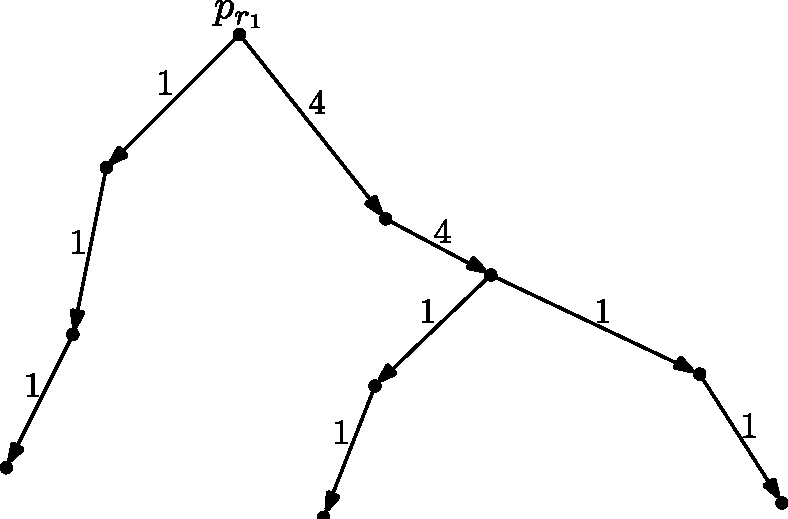
\includegraphics[width=\linewidth]{min_sum_tree_1.pdf}
	\end{subfigure}%
	\begin{subfigure}{.5\textwidth}
		\centering
		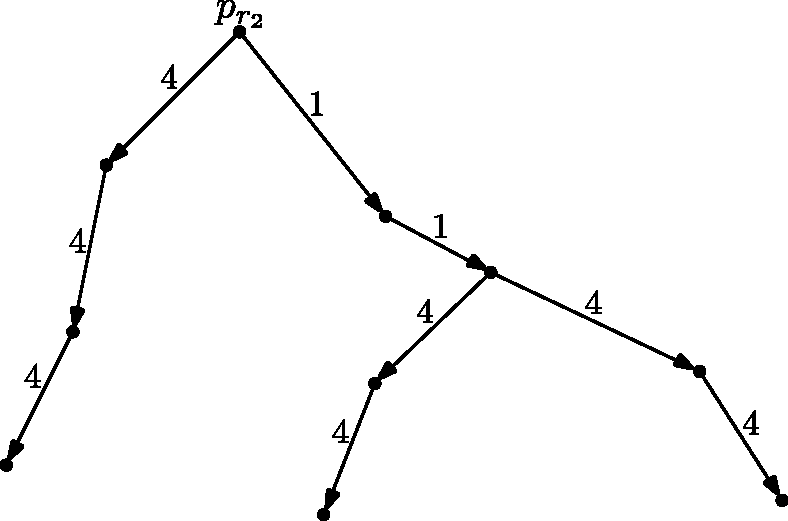
\includegraphics[width=\linewidth]{min_sum_tree_2.pdf}
	\end{subfigure}
	\caption{
	Eine Skizze von $H$. Jeder Knoten in $H$ repräsentiert genau eine Knoten-Platzierung.
	Dabei repräsentiert $\widehat{p_r}$ konkret die $\varepsilon$-Platzierung von $r$, welche in $\widehat{G_2}$ liegt und analog
	repräsentiert $\widetilde{p_r}$ die $\varepsilon$-Platzierung von $r$, welche in $\widetilde{G_2}$ liegt.
	Wir haben $H$ hierbei so skizziert, dass sich die durch $H$ repräsentierten Knoten-Platzierungen aus ihrer Lage ergeben, welche
	der Einbettung von $G_1$ in Abbildung \ref{min_sum_tree_0} nachempfunden ist.
	Die Kanten von $H$ sind bereits gewichtet und kennzeichnen die minimalen Kosten - gemäß des (schwachen) Fréchet-Abstands -
	einer Kanten-Platzierung für eine Auswahl zweier (schwach) voneinander erreichbarer Knoten-Platzierungen.
	\\
	\\
	Quelle: Eigene Darstellung.
	}
	\label{min_sum_tree_1}
\end{figure}

Nun beginnen wir, die Knoten in $G_1$ zu bearbeiten, deren Nachfahren allesamt Blätter sind. Initial sind dies die Knoten $v_1, v_2, v_3$ (siehe Abbildung \ref{min_sum_tree_0}).
Bei den $\varepsilon$-Platzierungen der Knoten behalten wir die Konvention bei, dass wir für einen Knoten $v_i \in V_1$ mit $\widehat{p_{v_i}}$ die $\varepsilon$-Platzierung von $v_i$ innerhalb
von $\widehat{G_2}$ und analog mit $\widetilde{p_{v_i}}$ die $\varepsilon$-Platzierung von $v_i$ innerhalb $\widetilde{G_2}$ kennzeichnen. Da das Gewicht aller Knoten-Platzierungen initial auf 0 gesetzt ist,
sind zur Berechnung der Gewichte der Knoten-Platzierungen von $v_1,v_2,v_3$ lediglich die durch entsprechenden gewichteten Kanten in $H$ zu betrachten (siehe Abbildung \ref{min_sum_tree_iteration_0}).

\begin{figure}[H]
	\centering
	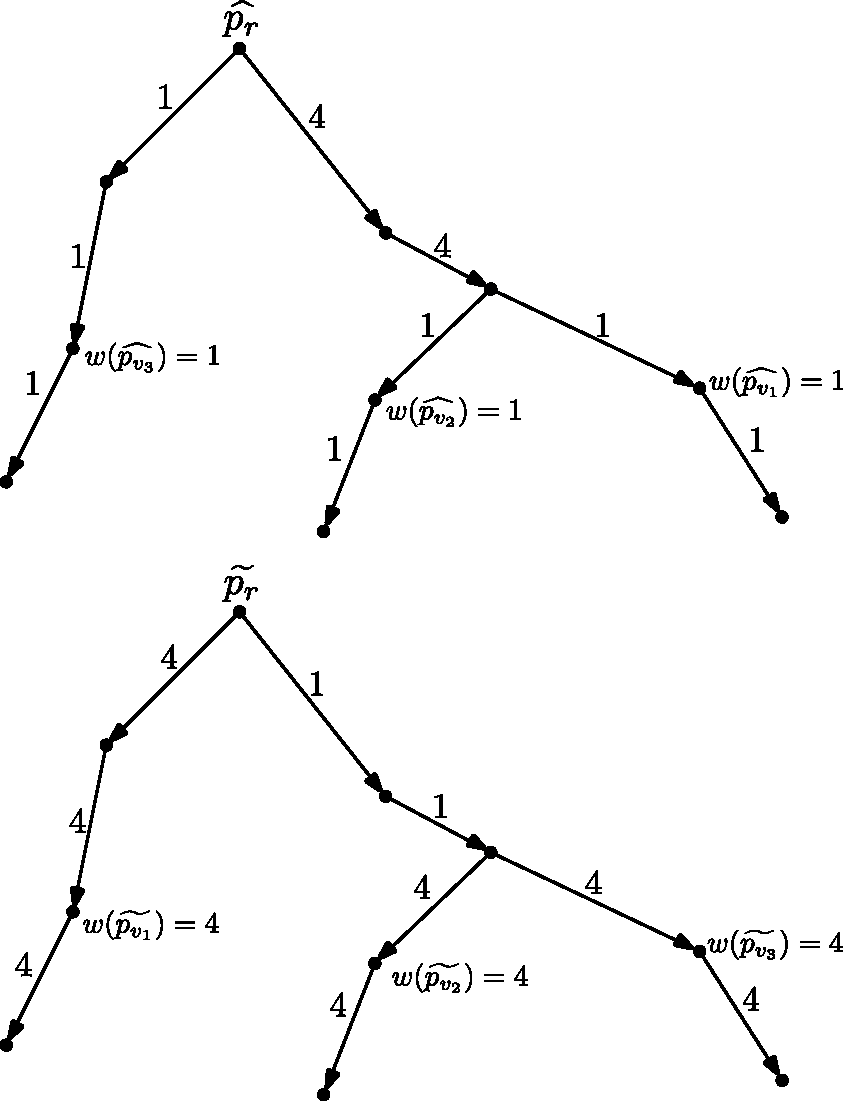
\includegraphics[width=0.8\linewidth]{min_sum_tree_h_0.pdf}
	\caption{
		Nachdem die Knoten $v_1,v_2,v_3$ bearbeitet wurden, sind die Gewichte aller ihrer $\varepsilon$-Platzierungen berechnet.
	}
	\label{min_sum_tree_iteration_0}
\end{figure}

Anschließend sind die Knoten $v_4$ und $v_5$ in dem aktualisierten Graphen $G_1^3$ diejenigen Knoten, deren Nachfahren Blätter sind.

$w(\widehat{p_{v_5}})$ berechnet sich zum Beispiel konkret entsprechend der Gleichung (\ref{optimal placements}) über
\begin{equation} \label{min_sum_weight_example}
	\begin{split}
		w(\widehat{p_{v_5}}) & = w(\widehat{p_{v_2}}) + w_H(\widehat{p_{v_5}}, \widehat{p_{v_2}}) + w(\widehat{p_{v_3}}) + w_H(\widehat{p_{v_5}}, \widehat{p_{v_3}}) \\
		& = 1 + 1 + 1 + 1 \\
		& = 4
	\end{split}
\end{equation}

Da in diesem Beispiel für alle Knoten-Platzierungen jeweils genau eine (schwach) erreichbare Knoten-Platzierung existiert, brauchen wir grundsätzlich - und explizit in in Gleichung (\ref{min_sum_weight_example}) -
kein Minimum aus mehreren Möglichkeiten berechnen.
\\
\\
Nachdem alle inneren Knoten von $G_1$ bearbeitet wurden, steht nur noch die Bearbeitung des Wurzelknotens $r$ aus.
Die bis dahin berechneten Gewichte sind in Abbildung \ref{min_sum_tree_h_1} notiert.

\begin{figure}[H]
	\centering
	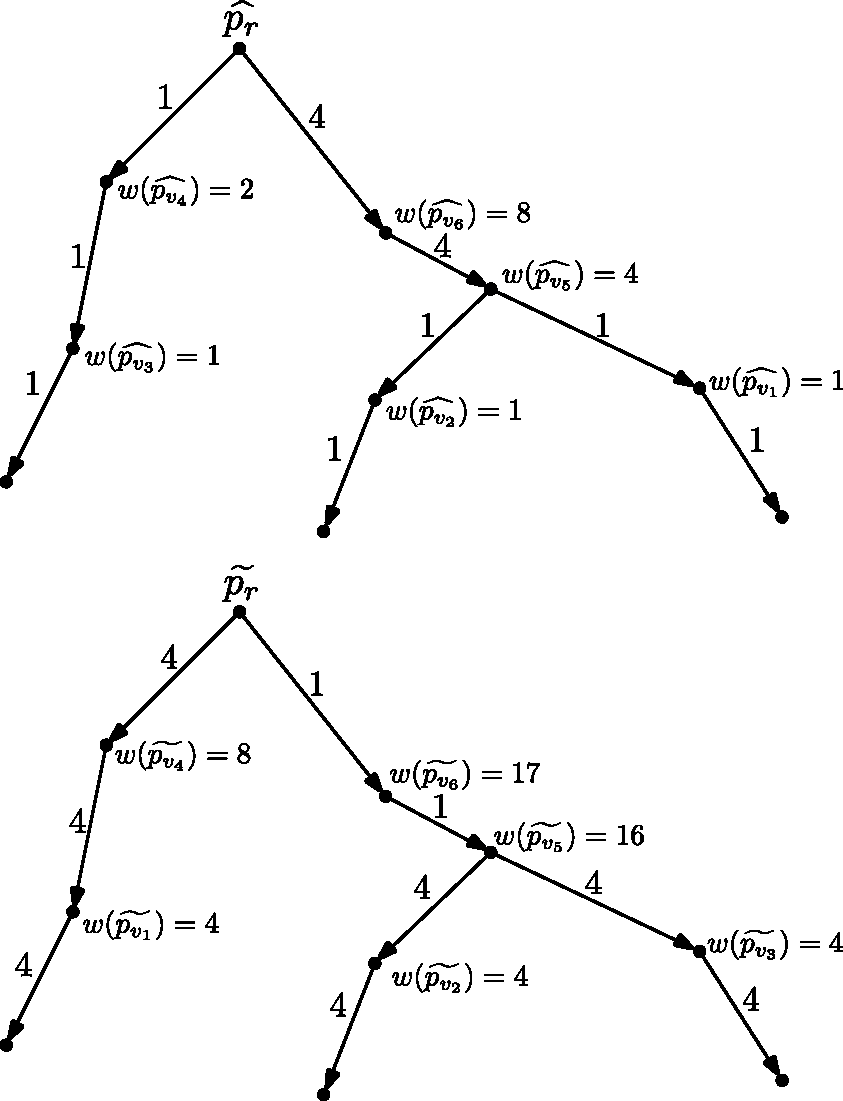
\includegraphics[width=.8\textwidth]{min_sum_tree_h_1.pdf}
	\caption{
		Alle berechneten Gewichte von $\varepsilon$-Platzierungen der inneren Knoten ($v_i$) von $G_1$.
	}
    \label{min_sum_tree_h_1}
\end{figure}

Für die $\varepsilon$-Platzierungen von $r$ berechnen wir
\begin{equation} \label{min_sum_weight_root_hat}
	\begin{split}
		w(\widehat{p_{r}}) & = w(\widehat{p_{v_4}}) + w_H(\widehat{p_{r}}, \widehat{p_{v_4}}) + w(\widehat{p_{v_6}}) + w_H(\widehat{p_{r}}, \widehat{p_{v_6}}) \\
		& = 2 + 1 + 8 + 4 \\
		& = 15
	\end{split}
\end{equation}
und
\begin{equation} \label{min_sum_weight_root_tilde}
	\begin{split}
		w(\widetilde{p_{r}}) & = w(\widetilde{p_{v_4}}) + w_H(\widetilde{p_{r}}, \widetilde{p_{v_4}}) + w(\widetilde{p_{v_6}}) + w_H(\widetilde{p_{r}}, \widetilde{p_{v_6}}) \\
		& = 8 + 4 + 17 + 1 \\
		& = 30
	\end{split}
\end{equation}

Damit ist Min-Sum$_{(w)F}(G_1,G_2) = 15$ und die Graph-Zuordnung $s$, die $w(\widetilde{p_{r}}) = 15$ realisiert, ist eine Min-Sum$_{(w)F}$ Zuordnung.
In unserem Beispiel ist das Bild von $s$ gerade $\widehat{G_2}$.

\newpage
\section{Komplexität} \label{Kapitel 4}

\subsubsection{NP-Schwerheit von Min-Sum$_{(w)F}$}

Abschließend wollen wir zeigen, dass die Berechnung des Min-Sum$_{(w)F}$ Abstands ohne Bedingungen an die Graphen $G_1$ und $G_2$ im Allgemeinen
NP-schwer ist. Ein für die Konstruktion des Beweises ähnliches Setting finden wir in [2] (Seite), wo die NP-Schwerheit des Graph-Abstands
über eine Reduktion von \textit{Binary Constraint Satifaction Problem (CSP)} gezeigt wird.
Hier orientieren wir uns im Wesentlichen an der oben genannten Konstruktion aus [2].

\begin{Def}
	Binary Constraint Satisfaction Problem
	Ein \textit{Binary Constraint Satisfaction Problem} beschreibt folgendes Entscheidungsproblem:
	\\
	Gegeben eine Instanz $\langle X,D,C \rangle$ bestehend aus
	$$ \text{einer Menge von \textit{Variablen }}X = \{x_1, x_2, ..., x_n\}, $$
	$$ \text{einer Menge von \textit{Domänen }}D = \{D_1, D_2, ..., D_n\}, $$
	$$ \text{und einer Menge von \textit{Bedingungen }}C = \{C_1, C_2, ..., C_k\}. $$
	Für jede Variable $ x_i \in X$ beschreibt ihre Domäne $ D_i \in D$ die Menge ihrer möglichen Wertzuweisungen.
	Eine Bedingung $C_{i,j} \in C$ spezifiert für je zwei unterschiedliche Variablen $x_i, x_j \in X$ eine Relation $R_{C_{i,j}}$ $\subseteq D_i \times D_j$.
	Wir nennen ein Wertepaar $(d_i, d_j) \in D_i \times D_j$ für eine vorhandene Bedingung $C_{i,j}$ an die Variablen $x_i,x_j$ \textit{zulässig}, wenn $(d_i,d_j) \in R_{C_{i,j}}$,
	ansonsten \textit{verletzt} das Wertepaar $(d_i, d_j)$ die Bedingung $C_{i,j}$ und wir nennen $(d_i,d_j)$ \textit{unzulässig}.
	\\
	Die Fragestellung ist nun, ob alle Variablen einem Wert aus ihrer Domäne zugewiesen werden können, so dass alle mit Bedingungen versehenden Wertepaare zulässig sind.
	In diesem Falle nennen wir $\langle X,D,C \rangle$ \textit{lösbar}.
	\\
	\\
	Für die allgemeine Komplexität der Klasse von \textit{Constraint Satisfaction Problems} und insbesondere des
	\textit{Binary Constraint Satisfaction Problems} siehe zum Beispiel \cite{Karp}.
\end{Def}

\begin{Satz} \label{Satz NP-Schwerheit}
	Theorem: Seien $G_1$ und $G_2$ geometrische Graphen und sei $\varepsilon \geq 0$.
	Das Entscheidungsproblem $$ \textit{Min-Sum}_{(w)F}(G_1, G_2) \leq  \varepsilon $$ ist NP-schwer.
\end{Satz}

\begin{proof}
Sei $\langle X,D,C \rangle$ ein beliebiges Binary Constraint Satisfaction Problem.
\\
\\
Wir repräsentieren jede Variable $x_i \in X$ durch einen Knoten $v_i \in V_1$ in $G_1$ und für jede Bedingung $C_{i,j}$ an die Variablen $x_i, x_j$
hat $G_1$ die Kante $\{v_i, v_j\}$. Wir setzen $\varepsilon = |E_1|$.
\\
Wir betten $G_1$ so in die euklidische Ebene ein, dass sich für je zwei Knoten $v_i,v_j$ ihre $\varepsilon$-Bälle nicht berühren und
sich der $\varepsilon$-Schlauch einer Kante $e \in E_1$ genau dann mit dem $\varepsilon$-Ball eines Knotens $v \in V_1$ überlappt, wenn $e$ und $v$ inzident sind.
\\
\\
Eine solche Einbettung für $G_1$ lässt sich zum Beispiel realisieren, indem wir die Knoten in $G_1$ (gleichmäßig) auf einem Kreis mit entsprechend großem Radius verteilen.
\\
Jeder Wert $d_{i,a} \in D_i$ wird durch einen Knoten $u_{i,a}$ in $G_2$ repräsentiert und wir betten $u_{i,a}$ beliebig innerhalb des 1-Balles $B_1(v_i)$ von $v_i$ ein.
Für jedes Wertepaar $d_{i,a} \in D_i, d_{j,b} \in D_j$ enthält $G_2$ genau dann die Kante $\{u_{i,a},u_{j,b}\}$, wenn die Wertekombination $(d_{i,a},d_{j,b})$
zulässig ist.
\\
Alle einzubettenen Kanten von $G_1$ und $G_2$ ergeben sich explizit (als Geradenstücke) zwischen den entsprechenden Knoten-Einbettungen.
Insgesamt behaupten wir, dass sich die oben beschriebene Einbettung von $G_1$ und $G_2$ in Polynomialzeit realisieren lässt.
Für ein kleines Beispiel der beschriebenen Konstruktion referenzieren wir auf Abbildung \ref{chapter_4_construction}.

\begin{figure}[H]
	\centering
	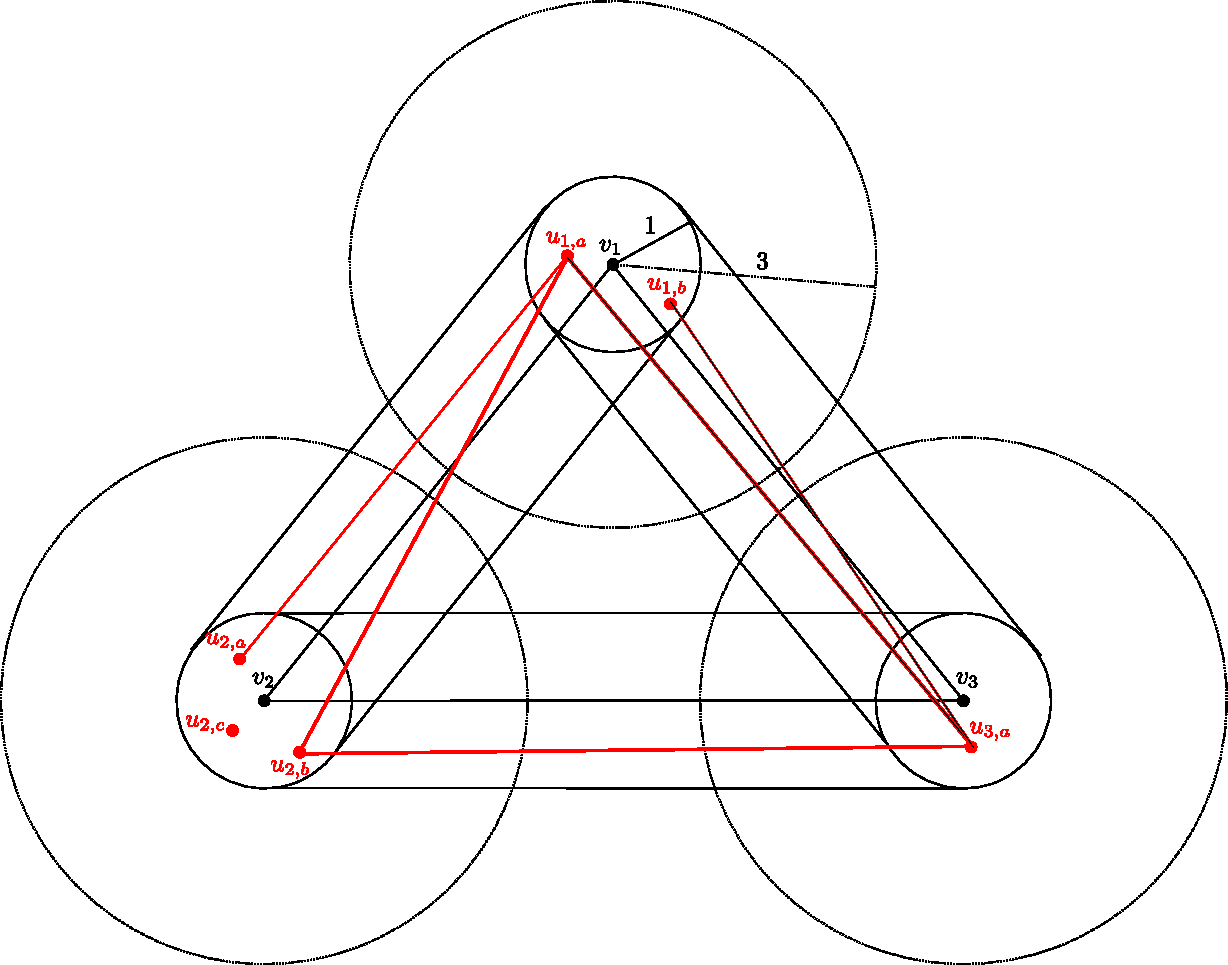
\includegraphics[width=\linewidth]{chapter_4_construction.pdf}
	\caption{
		Eine Einbettung von $G_1$ und $G_2$ nach oben beschriebener Konstruktion. Zugrunde liegt die Instanz $\langle X,D,C \rangle$ mit: $X=\{x_1,x_2,x_3\}$,
		$D_1=\{d_{1,a},d_{1,b}\}$, $D_2=\{d_{2,a},d_{2,b},d_{2,c}\}$, $D_3=\{d_{3,a}\}$ und den Bedingungen $C_{1,2},C_{1,3},C_{2,3},$ mit den Relationen
		$R_{C_{1,2}} = \{(d_{1,a},d_{2,a}),(d_{1,a},d_{2,b})\}, R_{C_{1,3}} = \{(d_{1,a},d_{3,a})\}$ und $R_{C_{2,3}} = \{(d_{2,b},d_{3,a})\}$.
		Es ist $\varepsilon = |E_1| = 3$ und die hervorgehobene Kurve kennzeichnet das Bild einer (schwachen) 1-Platzierung von $G_1$. Offensichtlich ist
		damit Min-Sum$_{(w)F}(G_1,G_2) \leq \varepsilon$ und die durch die Min-Sum$_{(w)F}$ Abbildung implizierte Auswahl von Werten
		$\{d_{1,a}, d_{2,b}, d_{3,a}\}$ ist eine Lösung von $\langle X,D,C \rangle$.
		\\
		\\
		Quelle: Eigene Darstellung
	}
	\label{chapter_4_construction}
\end{figure}

Wir wollen nun zeigen, dass
$$ \min_{s: G_1 \to G_2} \sum_{e \in E_1} \delta_{(w)F}(e, s(e)) \leq \varepsilon \iff \langle X,D,C \rangle \text{ ist lösbar}$$
"$\Leftarrow$":
\\
Sei $\langle X,D,C \rangle$ lösbar.
\\
Dann existiert eine Wertezuweisung $(\tilde{d_1},\tilde{d_2},...,\tilde{d_n}) \in {D_1 \times D_2 \times ... \times D_n},$ welche keine der Bedingungen verletzt.
\\
\\
Wir definieren eine Abbildung $\tilde{s}:G_1 \to G_2$ mit $\tilde{s}(v_i) = u_{\tilde{d_i}}$.
Nach Konstruktion von $G_2$ existiert für jedes $\tilde{d_i}$ ein entsprechendes $u_{\tilde{d_i}} \in G_2$.
\\
Ferner existiert für eine beliebige Kante $\{v_i, v_j\} \in E_1$ die Kante $\{u_{\tilde{d_i}}, u_{\tilde{d_j}}\} \in E_2$ und
und da das mit $\{u_{\tilde{d_i}}, u_{\tilde{d_j}}\}$ assoziierte Wertepaar $(\tilde{d_i},\tilde{d_j})$ per Vorraussetzung zulässig ist,
liegt $\{u_{\tilde{d_i}}, u_{\tilde{d_j}}\}$ innerhalb von $T_1(\{v_i, v_j\}$ und die Randpunkte liegen respektive innerhalb von $B_1(v_i)$ und $B_1(v_j)$.
Damit ist grundsätzlich $\delta_{(w)F}(\{v_i, v_j\}\,\{u_{\tilde{d_i}}, u_{\tilde{d_j}}\}) \leq 1$ (siehe dazu auch \ref{Definition Fréchet-Abstand}).
\\
\\
Wir erweitern $\tilde{s}$ nun insofern, dass $\{v_i, v_j\}$ durch $\tilde{s}$ so auf $\{u_{\tilde{d_i}}, u_{\tilde{d_j}}\}$ abgebildet wird,
dass $\tilde{s}$ den Flaschenhals-Abstand von $\delta_{(w)F}(\{v_i, v_j\}, s(\{v_i, v_j\}) \leq 1$ realisiert.
Bilden wir jede Kante von $G_1$ auf diese Weise auf $G_2$ ab, so ist $\tilde{s}$ eine Graph-Zuordnung und $\delta_{(w)F}(e, \tilde{s}) \leq 1$ für jedes $e \in E_1$,
also ist $\tilde{s}$ eine 1-Platzierung von $G_1$.
\\
\\
Damit ist
\begin{equation} \label{beweis_1}
	\sum_{e \in E_1} \delta_{(w)F}(e, \tilde{s}(e)) \leq \varepsilon
\end{equation}
\\
Über die Identitäten $$\min_{s: G_1 \to G_2} \sum_{e \in E_1} \delta_{(w)F}(e, s(e)) \leq \sum_{e \in E_1} \delta_{(w)F}(e,\tilde{s}(e)) $$
und (\ref{beweis_1}) erhalten wir insgesamt
$$\min_{s: G_1 \to G_2} \sum_{e \in E_1} \delta_{(w)F}(e, s(e)) \leq \varepsilon .$$
\\
\\
"$\Rightarrow$":
\\
Sei $$\min_{s: G_1 \to G_2} \sum_{e \in E_1} \delta_{(w)F}(e, s(e)) \leq {\varepsilon}.$$
\\
\\
So ist $s(e)$ für alle $e \in E_1$ eine (schwache) $\varepsilon$-Platzierung von $e$,
da ansonsten $\delta_{(w)F}(\tilde{e}, s(\tilde{e})) > \varepsilon$ für ein $\tilde{e} \in E_1$ und damit insbesondere $\sum_{{e}\in E_1} \delta_{(w)F}(e, s(e)) > \varepsilon$.
(*)
\\
\\
Zusätzlich wollen wir argumentieren, dass $s(e)$ für alle $e \in E_1$ eine (schwache) 1-Platzierung von $e$ ist.

Wir haben bereits argumentiert, dass jedes Bild einer Kante von $G_1$ unter $s$ eine $\varepsilon$-Platzierung sein muss.
Damit liegen die Randpunkte von $s(e)$ insbesondere innerhalb der $\varepsilon$-Platzierungen der zu $e$ inzidenten Knoten.
Wenn $s(e)$ eine $\varepsilon$-Platzierung von $e$ ist, so muss $s(e)$ insbesondere auch eine 1-Platzierung von $e$ sein.
\\
Dies ergibt sich aus der Vorraussetzung, dass $s$ eine Min-Sum$_{(w)F}$ Zuordnung ist und sich daher unter Berücksichtigung Konstruktion
von $G_1$ und $G_2$ jede $\varepsilon$-Platzierung von $e$ sich grundsätzlich als 1-Platzierung von $e$ realisieren lässt.
\\
Denn die Randpunkte von $s(e)$ lassen sich so innerhalb der $\varepsilon$-Bälle verschieben, dass sie innerhalb der entsprechenden 1-Bälle liegen
und da alle Kanten von $G_2$ innerhalb von $T_{\varepsilon}(e)$
per Konstruktion insbesondere als Geradenstücke innerhalb von $T_1(e)$ liegen, existiert in $G_2$ eine 1-Platzierung von $e$.
\\
\\
Damit ist für eine Kante $\{v_i, v_j\} \in E_1$ ihr Bild $s(\{v_i, v_j\})$ stets eine 1-Platzierung von $\{v_i, v_j\}$. (**)
\\
\\
Im Falle des Fréchet-Abstands gilt damit, dass wir durch eine $\text{Min-Sum}_F$ Zuordnung $s: G_1 \to G_2$ das Bild $s(\{v_i, v_j\})$ einer Kante
eindeutig mit einer Kante $\{u_{i,a}, u_{j,b}\} \in E_2$ identifizieren können. Gemeint ist damit genau die Kante, welche
die entsprechenden $1$-Platzierungen der Knoten $v_i$ und $v_j$ verbindet und in $T_1(\{v_i, v_j\})$ liegt. Die Eindeutigkeit dieser Kante folgt direkt aus der
Konstruktion von $G_2$.
\\
Durch (**) ist gewährleistet, dass für die Kante $\{u_{i,a}, u_{j,b}\} \in E_2$, ihren assoziierten Wertezuweisungen $(d_{i,a}, d_{j,b}) \in D_i \times D_j$
und die Bedingung $C_{i,j} \in C$ an die Variablen $x_i, x_j$ gilt:
$$(d_{i,a},d_{j,b}) \in R_{C_{i,j}}$$
Damit ist im Falle des Fréchet-Abstands $\langle X,D,C \rangle$ erfüllbar.
\\
\\
Für den schwachen Fréchet-Abstand gilt das Argument, dass wir das Bild einer Kante in $G_1$ unter $s$ eindeutig mit einer Kante in $G_2$ identifizieren können, allgemein nicht.

Dies liegt daran, dass grundsätzlich jedes beliebige Knotenpaar $u_{i}, u_{j} \in V_2$ mit $u_{i} \in B_1(v_i)$, $u_{j} \in B_1(v_j)$ eine Kante in $G_2$ haben kann.
\\
So existieren einfache Wege in $G_2$ bestehendend aus mindestens 3 Kanten innerhalb von $T_1(\{v_i, v_j\}$, deren Startpunkt in $B_1(v_i)$ und deren Endpunkt in $B_1(v_j)$ liegt.
Ein solcher Weg $W$ ist dabei - da er bedingt durch die Konstruktion von $G_2$ vollständig innerhalb von $T_1(\{v_i, v_j\}$ liegt - eine schwache 1-Platzierung der Kante $\{v_i, v_j\}$,
also $\delta_{wF}(\{v_i, v_j\}, W) \leq 1$.

\begin{figure}[H]
    \centering
    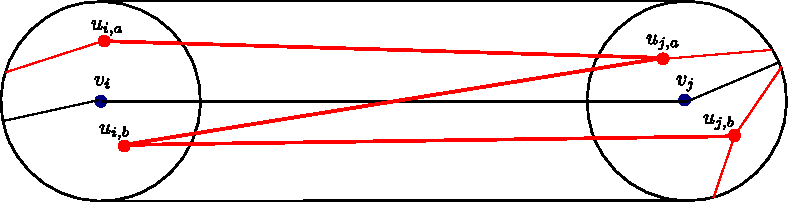
\includegraphics[width=0.8\textwidth]{chapter_4_example_0.pdf}
    \caption{Durch die Hervorhebung haben wir das Bild eines Weges $W$ in $G_2$ markiert, welcher zwei 1-Platzierungen schwach miteinander verbindet.
	Für den schwachen Fréchet-Abstand genügt dabei die Tatsache, dass $W$ vollständig in $T_1(\{v_i,v_j\})$ liegt.
	Die mit der Kanten-Platzierung assoziierten Knoten $u_{i,a},u_{j,b}$ repräsentieren allerdings offensichtlich keine gültige Wertezuweisung für die Variablen $x_i,x_j$.
	Im Allgemeinen garantiert uns für den schwachen Fréchet-Abstand somit Min-Sum$_{wF}(G_1,G_2) \leq \varepsilon$ noch keine Lösbarkeit von $\langle X,D,C \rangle$.
	\\
	\\
	Quelle: Eigene Darstellung
	}
\end{figure}

Um diesen Fall auszuschließen und ein ähnliches Szenario wie für den Fréchet-Abstand zu gewährleisten, fügen wir mittig auf jeder Kante $\{v_i, v_j\} \in E_1$
einen zusätzlichen Knoten $v_{ij}$ in $G_1$ ein, so dass $B_1(v_{ij}) \cap B_1(v_i) = B_1(v_{ij}) \cap B_1(v_j) = \emptyset$ (siehe dazu Abbildung \ref{fig:chapter_4_example_1}).
Dafür ist es unter Umständen notwendig, initial ein größeres $\varepsilon$ zu wählen, damit die beschriebene Konstruktion (auch für $m_1 \leq 3$) stets gelingt.
\\
\\
\begin{figure}[H]
    \centering
    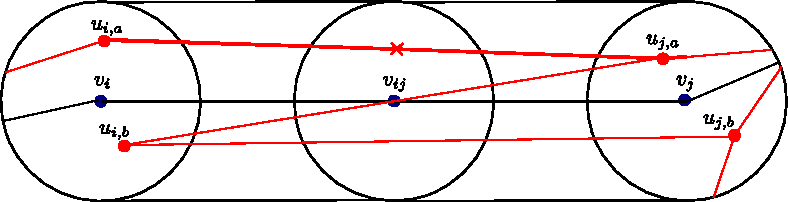
\includegraphics[width=0.8\textwidth]{chapter_4_example_1.pdf}
    \caption{
	Die Kante $\{v_i, v_j\}$ zerfällt nach dem Hinzufügen von $v_{ij}$ in die zwei Kanten $\{v_i, v_{ij}\}$, $\{v_{ij},v_j\}$.
	$s(v_{ij})$ ist in der Abbildung durch ein rotes Kreuz gekennzeichnet.
	Jede Kante in $G_2$ von $B_1(v_i)$ nach $B_1(v_j)$ induziert eine eindeutige 1-Platzierung
	des Knotens $v_{ij}$. Da $B_1(v_{ij})$ keine Knoten von $G_2$ enthält, ist die Konkatenation der Bilder von $\{v_i,v_{ij}\}$ und $\{v_{ij},v_j\}$
	unter $s$ eindeutig mit einer Kante in $G_2$ identifizierbar.
	\\
	\\
	Quelle: Eigene Darstellung
	}
    \label{fig:chapter_4_example_1}
\end{figure}

Wir bezeichnen mit $\tilde{G_1}=(\tilde{V_1}, \tilde{E_1})$ den Graphen, den wir durch die oben beschriebene Transformation erhalten.
\\
\\
Gilt nun
$$ \min_{s: \tilde{G_1} \to G_2} \sum_{e \in E_1} \delta_{wF}(e, s(e)) \leq 2m_1, $$
so erhalten wir für jede Kante $\{v_i, v_j\} \in E_1$ und ihre Zerlegung $\{v_i, v_{ij}\},\{v_{ij}, v_j\} \in \tilde{E_1}$
über $s(\{v_i, v_{ij}\})$ und $s(\{v_{ij}, v_j\})$ die eindeutige, assoziierte Kante $\{u_{i,a}, u_{i,b}\} \in E_2$.
Die durch $\{u_{i,a}, u_{j,b}\} \in E_2$ repräsentierte Wertezuweisung $(d_{i,a}, d_{j,b})$ verletzt dabei nicht die Bedingung an die
durch $v_i$ und $v_j$ repräsentierten Variablen $x_i, x_j$, und ist damit gültig.
\\
\\
Damit ist $\langle X,D,C \rangle$ lösbar.
\end{proof}

\newpage

\section{Ausblick}
In dieser Arbeit haben wir uns, motiviert durch das Ziel optimale Zuordnungen auf geometrischen Graphen zu untersuchen, mit dem
Min-Sum$_{(w)F}$ Abstands beschäftigt. Dabei haben wir Komplexität für allgemeine
Graphen geklärt und - falls $G_1$ ein Baum ist und wir die Menge der Graph-Zuordnungen (wie in \ref{Einschränkungen} beschrieben) einschränken -
einen Polynomialzeit-Algorithmus zur Berechnung dieses Abstandsmaßes beschrieben.
\\
Dabei verbleiben noch einige offene Fragen bezüglich der Komplexität.
Buchin et al. \cite{Buchin} gehen davon aus dass die Berechnung des Min-Sum-$_{(w)F}$ Abstands auch auf planaren Graphen und
auf Bäumen ohne die notwendige Einschränkung (aus \ref{Zweite Einschränkung}) NP-schwer ist.
Formale Beweise dieser Annahmen stehen dabei noch aus.
\\
\\
Allgemein beschreibt der Min-Sum-Graph-Abstand$_{dist}$ eine ganze Klasse von Abstandsmaßen auf Graphen, deren Mitglieder sich durch die Wahl
eines geeigneten Abstandsmaßes für die Gewichtung der Kanten-Zuordnungen unterscheiden.
Grundsätzlich sind die Eigenschaften des Min-Sum-Graph-Abstands unter anderen Abstandsmaßen zu betrachten. Hier bietet sich zum Beispiel der
diskrete Fréchet-Abstand als geeigneter Kandidat an. Wir behaupten, dass wir aufgrund seiner inherenten Eigenschaft die in $\ref{Zweite Einschränkung}$
geforderten Fixpunkte zur Gewährleistung einer polynomiellen Laufzeit der Berechnung nicht benötigen.
\\
\\
Wir haben bei unserer Betrachtung des Min-Sum$_{(w)F}$ Abstands bisher nur ein Mitglied dieser oben beschriebenen Klasse genauer betrachtet und
damit ledglich einen kleinen Exkurs in den Raum der offenen Möglichkeiten gewagt.
\newpage\null\thispagestyle{empty}\newpage
%   Eventuell eine Leerseite vor der Literaturangabe, falls diese sonst auf einer Rückseite angegeben würde. (Seitennummer muss ungerade sein!)

\begin{thebibliography}{3}
	\bibitem{Buchin}
		Maike Buchin, Bernhard Kilgus. Distance Measures for Embedded Graphs - Optimal Graph Mappings.
		\textit{European Workshop on Computational Gemoetry,} 2020.

	\bibitem{Akitaya}
		Hugo Akitaya, Maike Buchin, Bernhard Kilgus, Stef Sijben, Carola Wenk. Distance measures for embedded graphs
		\textit{Computational Geometry,} Volume 95, 2021.

	\bibitem{Alt}
		Hemlut Alt, Michael Godau. Computing the Fréchet distance between two polygonal curves.
		\textit{Int. Journal of Computational Geometry and Applications,} 5:75-91, 1995.

	\bibitem{Alt2}
		Helmut Alt, Alon Efrat, Günter Rote, and Carola Wenk. Matching planar maps.
		\textit{Journal of Algorithms, 49(2):262 – 283, 2003.}

	\bibitem{Ref1}
		Joachim Gudmundsson, Martin P. Seybold, Sampson Wong. Map matching queries on realistic input graphs under the Fréchet distance.
		\textit{In Proceedings of the 2023 Annual ACM-SIAM Symposium on Discrete Algorithms (SODA) (pp. 1464-1492). Society for Industrial and Applied Mathematics, 2023.}

	\bibitem{Ref2}
		Kevin Buchin, Maike Buchin, Joachim Gudmundsson, Aleksandr Popov, Sampson Wong. Map Matching Queries Under Fréchet Distance on Low-Density Spanners.
		\textit{In The 39th European Workshop on Computational Geometry, 2023.}
	\bibitem{Karp}
		Karp, Richard M. Reducibility among combinatorial problems.
		\textit{Springer Berlin Heidelberg, 2010.}

\end{thebibliography}

% Symbolverzeichnis definieren
%\nomenclature{$c$}{Speed of light in a vacuum inertial frame}
%\nomenclature{$h$}{Planck constant}

%\printnomenclature
\end{document}
